\documentclass[pageno]{jpaper}


\usepackage{graphicx}
\usepackage{subfig}
%Removing the geometry package used for Tighter Format
%\usepackage{geometry}
%\usepackage{times}
\usepackage{textcomp}
\usepackage{multirow}
\usepackage{framed}
\usepackage{amsmath}
\usepackage{listings}

% \usepackage[hyphens]{url}
\PassOptionsToPackage{hyphens}{url}
\usepackage{hyperref}
%\usepackage{hyperref}
\usepackage{enumitem}
\usepackage{amssymb}

%Used only for breaking hypenated URLs
\usepackage{etoolbox}
\gappto{\UrlBreaks}{\UrlOrds}
%

\hypersetup{breaklinks=true}

\urlstyle{same}

%\usepackage[activate={true,nocompatibility},final,tracking=true,kerning=true,spacing=true,factor=1100,stretch=20,shrink=20]{microtype}


% \newcommand{\submissionnumber}{144}
% \newcommand{\sysname}{Il\'uvatar}
\newcommand{\D}{\emph{D}}
\newcommand{\Dmax}{\emph{D\_max}}
\newcommand{\T}{\emph{T}}
\newcommand{\VT}{\emph{VT}}
\newcommand{\GlobVT}{\emph{Global\_VT}}
\newcommand{\FinVT}{\todo{REMOVE: finish\_vt}}
% \newcommand{\QName}{MQ-FLQ}
% \newcommand{\QNameFull}{Multi-Queue Fair \& Local Queuing}
\newcommand{\QName}{MQFQ-Sticky}
\newcommand{\QNameFull}{\QName}
\newcommand{\batch}{\texttt{Batch}}
\newcommand{\naive}{\texttt{FCFS Naïve}}
\newcommand{\fcfs}{\texttt{FCFS}}

% \usepackage{tikz}

% \RequirePackage[normalem]{ulem}
% \RequirePackage{color}\definecolor{RED}{rgb}{1,0,0}\definecolor{BLUE}{rgb}{0,0,1}
\providecommand{\DIFadd}[1]{{\protect\color{blue}\uwave{#1}}}
\providecommand{\DIFdel}[1]{{\protect\color{red}\sout{#1}}}
%DIF SAFE PREAMBLE
\providecommand{\DIFaddbegin}{}
\providecommand{\DIFaddend}{}
\providecommand{\DIFdelbegin}{}
\providecommand{\DIFdelend}{}
%DIF FLOATSAFE PREAMBLE
\providecommand{\DIFaddFL}[1]{\DIFadd{#1}}
\providecommand{\DIFdelFL}[1]{\DIFdel{#1}}
\providecommand{\DIFaddbeginFL}{}
\providecommand{\DIFaddendFL}{}
\providecommand{\DIFdelbeginFL}{}
\providecommand{\DIFdelendFL}{}
%DIF END PREAMBLE EXTENSION ADDED BY LATEXDIFF

\def\Section {\S}

\newcommand{\squishlist}{
 \begin{list}{$\bullet$}
  { \setlength{\itemsep}{0pt}
     \setlength{\parsep}{3pt}
     \setlength{\topsep}{3pt}
     \setlength{\partopsep}{0pt}
     \setlength{\leftmargin}{1.5em}
     \setlength{\labelwidth}{1em}
     \setlength{\labelsep}{0.5em} } }
	
\newcommand{\squishlisttwo}{
 \begin{list}{$\bullet$}
  { \setlength{\itemsep}{0pt}
     \setlength{\parsep}{0pt}
    \setlength{\topsep}{0pt}
    \setlength{\partopsep}{0pt}
    \setlength{\leftmargin}{2em}
    \setlength{\labelwidth}{1.5em}
    \setlength{\labelsep}{0.5em} } }

\newcommand{\squishend}{
  \end{list}  }

% \newcommand{\squishenum}{
%   \begin{enumerate}{$\bullet$}
%     { \setlength{\itemsep}{0pt}
%       \setlength{\parsep}{0pt}
%       \setlength{\topsep}{0pt}
%       \setlength{\partopsep}{0pt}
%       \setlength{\leftmargin}{2em}
%       \setlength{\labelwidth}{1.5em}
%       \setlength{\labelsep}{0.5em} } }
  
% \newcommand{\squishenumend}{
%   \end{enumerate}  }

\newcommand{\alert}[1] {\textcolor{red} {\textsc{#1}}}

\newcommand{\myfbox}[1] {\noindent \fbox{\parbox{0.5\textwidth} {#1}}}

\newcommand{\mhead}[1] {\noindent \textbf{#1.}}

\newcommand*\mean[1]{\overline{#1}}

\newcommand{\eat}[1]{}

\newcommand{\compresslist}{%
  \setlength{\itemsep}{1pt}%
  \setlength{\leftmargin}{1.5em}
  \setlength{\labelwidth}{1em}
  \setlength{\parskip}{0pt}%
  \setlength{\parsep}{0pt}%
%  \setlength{\itemindent}{-10pt}%
}

\newcommand{\myfigspace}[0]{-0.3cm}
\newcommand{\bigfigspace}[0]{-0.9cm}
\newcommand{\captionspace}[0]{-0.25cm}
\newcommand{\subsecspace}[0]{-0.1cm}
\newcommand{\largesubsecspace}[0]{-0.38cm}

\newcommand\prat[1]{\textcolor{red}{(Prateek: #1)}}

\newcommand{\quotes}[1]{``#1''}
\newcommand{\todo}[1]{\textcolor{orange}{TODO: #1}}
\newcommand{\alex}[1]{\textcolor{blue}{Alex: #1}}
% https://tex.stackexchange.com/a/7045
\newcommand*\circled[1]{\tikz[baseline=(char.base)]{
            \node[shape=circle,draw,inner sep=2pt] (char) {#1};}}


\newcommand{\funcname}[1]{\texttt{#1}}

\newcommand{\asplossubmissionnumber}{1225}

\usepackage[normalem]{ulem}


\begin{document}
%-------------------------------------------------------------------------------

\title{FaasCache: Keeping Serverless Computing Alive With Greedy-Dual Caching}

%don't want date printed
\date{}

% make title bold and 14 pt font (Latex default is non-bold, 16 pt)
\author{}

\maketitle 

\thispagestyle{empty}

\begin{abstract}

Functions as a Service (also called serverless computing) promises to revolutionize how applications use cloud resources. 
However, functions suffer from cold-start problems due to the overhead of initializing their code and data dependencies before they can start executing. 
Keeping functions alive and warm after they have finished execution can alleviate the cold-start overhead. 
Keep-alive policies must keep functions alive based on their resource and usage characteristics, which is challenging due to the diversity in FaaS workloads. 


Our insight is that keep-alive is analogous to caching.
Our caching-inspired Greedy-Dual keep-alive policy can be effective in reducing the cold-start overhead by more than $3\times$ compared to current approaches. 
Caching concepts such as reuse distances and hit-ratio curves can also be used for auto-scaled server resource provisioning, which can reduce the resource requirement of FaaS providers by $30\%$ for real-world dynamic workloads. 
We implement caching-based keep-alive and resource provisioning policies in our FaasCache system, which is based on OpenWhisk. 
We hope that our caching analogy opens the door to more principled and optimized keep-alive and resource provisioning techniques for future FaaS workloads and platforms. 



%%% Local Variables:
%%% mode: latex
%%% TeX-master: "paper"
%%% End:

\end{abstract}

%%%%%%%%%%%%%%%%%%%%%%%%%%%%%%%%%%%%%%%%%%%%%%%%%%

%hotcloud is 5 pages of text 
%\vspace*{\subsecspace}
\section{Introduction}
\vspace*{\subsecspace}
\section{Introduction}

Function as a Service (also called FaaS or serverless computing) is one of the fastest growing abstractions in cloud computing today with usage increasing by 2x in the past two years alone~\cite{wen2023rise}.
% Users create self-contained \textit{functions} whose lifecycle is orchestrated by the FaaS provider.  
Users are enticed by its dynamic scaling, low cost, and ease of management, as the lifecycle of self-contained \textit{functions} is orchestrated by the FaaS provider.
% Cloud providers benefit because functions use ephemeral resources unlike traditional virtual machines (VMs) and the provider has find-grained control over scheduling and placement.
Cloud providers leverage the ephemeral nature of functions into fine-grained control over scheduling, placement, and resource allocation.

% 1)
Current FaaS applications are limited by the capabilities exposed by providers, mostly consisting of short-running functions~\cite{shahrad2020serverless} using limited compute.
% Functions are given limited CPU resources and have no way efficient of coordinating with one another, precluding classic parallel computing.
Providers have not exposed GPUs or other parallel processing paradigms to their serverless platforms, a need for which is growing as users migrate new, intensive, workflows to cloud FaaS.
These applications see a \emph{minimum} 2.5x throughput improvement when accelerated, strong encouragement to enable such devices in serverless platforms.

% 2-3)
Accomplishing this transition requires the control plane to address several resource management problems.
Achieving high device utilization and low latency require device multiplexing~\cite{pemberton2022kernel, ng2023paella, fingler2022dgsf, gu2023fast}, but unmodified functions preclude such sharing of GPU resources.
% To make matters more complicated, GPU resources are managed by an esoteric device driver that isn't controllable by the OS.
Once a function is given access to the GPU, it can allocate the entire memory range or hog compute in a run-to-completion model.
% Idle periods mean allocated resources on the GPU are blocked off, other functions being unable to use them for their executions.
% Removing containers to release held resources results in heavy churn and increased latency from the repeated container initialization.
Swapping functions requires starting a new container, costing several seconds on the critical path, making the well-known \quotes{cold start} problem of FaaS an even larger latency bottleneck.
% We avoid cold starts by being the first to enable GPU keep-alive~\cite{faascache-asplos21} policies via GPU resource multiplexing.
Avoiding cold starts (i.e. a warm start) to get viable performance requires enabling GPU keep-alive~\cite{faascache-asplos21} policies via GPU resource multiplexing.

\begin{comment}
Machines used to host FaaS systems are expected to serve thousands of unique functions with low latency.
This is accomplished by running user function code inside a container (or VM), then keeping the container in memory but idle for future uses. 
A na\"ive adaption of this to the GPU problem would assign an entire GPU to each container for its lifetime.
Unfortunately an idle container then wastes GPU resources, and the limited number of GPUs per server leads to churn when we need to create a new container for another function.
% but this causes low utilization and high turnover when going to run a new function.
Virtualization for these devices exists, provisioning fixed slices of GPU resources to containers that they then have exclusive access to.
% This also results in low utilization, as nothing else can use that section when it is idle, and also limits the resources available to give to any one function that might take advantage of them.
While allowing more containers to exist concurrently, this solution does not address idleness and introduces a new limitation by reducing the maximum allocation any single function is allowed to make.
\end{comment}
  
% 4-6)
Multiplexed resources are not a performance panacea: the platform must now contend with function fairness and locality.
% The FaaS control plane must also guarantee that all functions will run in a timely and fair manner.
% GPUs must also be shared temporally 
Optimal performance is achieved by running one function repeatedly, as its data dependencies will be available on-device.
Yet a popular function can easily starve others of device time and violate fairness guarantees if not eventually blocked.
% Temporal GPU sharing between the highly heterogeneous serverless workloads must be balanced with execution \quotes{locality}.
New queuing policies tailored to the unique scenario of GPU-serverless computing must be designed to ensure fairness while maintaining high throughput.
% Warm hits, i.e. executing using an already existing container, have up to 100x lower latency compared to their cold counterparts.
% Such execution \quotes{locality} can only come 
% want warm starts.
% locality good -> 'batching'.
% but need spatial/temporal multiplexing as well.

% 7
Previous research work into enabling GPU acceleration in FaaS has focused on ML inference~\cite{pemberton2022kernel, ng2023paella, fingler2022dgsf, gu2023fast}; understandable given its popularity.
These approaches have abandoned the black-box nature of FaaS in favor of extremely fine-grained control of GPU usage and scheduling.
Supporting functions of all types is critical, as more use cases like scientific computing~\cite{kumanov2018serverless,hung2019rapid}, video encoding~\cite{ao2018sprocket, zhang2019video}, and optimization problems~\cite{aytekin2019harnessing,werner2018serverless,shankar2020serverless}, migrate to the platform.
% Our work uniquely enables all these to run natively with minimal overhead.
% Custom solutions have been proposed~\cite{}, but rely on targeted workloads or bespoke platforms, a general-purpose approach is needed.

% 7)
Given these known problems, in this work we seek to answer several research questions:
\begin{enumerate}[leftmargin=*]
  % \item Can we provide GPU acceleration to black-box, unmodified, serverless functions?
  % \item How can GPU support be integrated into high-performance FaaS control planes?
  \item Can we provide GPU acceleration to black-box, unmodified, serverless functions?
  \item Can we multiplex GPU resources between functions in a low overhead manner?
  \item How do we balance locality, fairness, and performance in the face of heterogeneous functions?
  % \item Is this possible without the cost of full virtualization?
\end{enumerate}
% \todo{Better RQs to frame novelty}

In this work, we propose and designed a series of techniques and policies that resolve all of these issues.
They enable black-box serverless functions to utilize GPUs for acceleration while concurrently sharing its resources.
We built our system on top of the \sysname~platform~\cite{fuerst2023iluvatar}, utilizing Nvidia's integration with Docker~\cite{docker-main}. %, but is generic to any accelerator or isolation system.
Importantly, they don't rely on specific hardware or software versioning support, and work on heterogeneous hardware regardless of age or capability. 

% \mhead{RQ1}
Starting from the lowest level component, we interpose an intercept shim between function code and the GPU driver.
Using this, we capture all memory allocation calls and transform them into Unified Virtual Memory (UVM)~\cite{nvidia-uvm} calls.
UVM memory allows applications to allocate beyond the device limits, letting the driver use host memory as swap space, migrating memory on demand. 
Once all allocations are converted to UVM memory, we use the shim to move memory between host and device under direction from the control plane.

% \mhead{RQ2}
Controlling memory positioning allows us to both oversubscribe device memory and keep containers warm while other functions execute on the GPU.
To enable multiple functions to run concurrently, a new queuing policy is required that better matches the new device's capabilities and workload characteristics.
We accomplish this with a modified implementation of a Mutli-Queue Fair Queue (MQFQ)~\cite{hedayati2019multi}, which prevents starvation, scales invocations across multiple GPUs, and minimizes execution overhead.
To prevent contention interference, we monitor device utilization using NVML~\cite{nvml} and track memory usage to throttle invocations.

With these controls we improve function latency by orders of magnitude over previous solutions and expand the pool of serverless applications.
In short, this work proposes the following enhancements to serverless computing:
\begin{enumerate}[leftmargin=*]
  \item We create a custom driver that intercepts function allocation calls to multiplex device memory.
  \item With no limit on device memory, we can keep idle containers resident, creating the first warm pool of GPU containers.
  \item Our memory management techniques allow us to reduce device pressure from idle functions, mitigating overcommitment overhead.
  \item We design a queuing policy that enables concurrent execution while ensuring fairness under heterogeneous workloads.
  % \item W
  % \item Benchmark suite of GPU-enabled serverless functions, including many non-machine learning applications.
\end{enumerate}

This paper is ordered as follows.
Section~\ref{sec:bg} covers background of serverless work and GPU virtualization.
Our motivation behind work is explained in detail in Section~\ref{sec:motiv}.
Section~\ref{sec:design} details our design of queuing, memory control, and resource management.
We examine the implementation of these pieces in Section~\ref{sec:impl}.
Lastly, Section~\ref{sec:eval} shows the effectiveness of our systems with a thorough experiment suite.
 

% The idea is to write this like a propogsal with the crux of the idea..


%\vspace*{\subsecspace}
\section{Background}
\vspace*{\subsecspace}
%Background and related work. 
%background on serverless platforms and keep-alive

% This is an introductory paragraph talking about serverless computing and some context. Seems repetitive wrt introduction? 
Serverless computing is now being provided by all large public cloud providers: Amazon Lambda, Google Functions, and Azure Functions are becoming an increasingly popular way to deploy applications on the cloud.  
Functions as a Service (FaaS) can also be realized on private clouds and dedicated clusters through the use of frameworks such as OpenWhisk~\cite{openwhisk}, OpenFaas~\cite{openfaas}, OpenLambda~\cite{hendrickson2016serverless}, etc. 
%
In this new cloud paradigm, users provide functions in languages such as Python, Javascript, Go, and others. 
%
The functions are executed by the FaaS platform, greatly simplifying resource management for the application. 



% Need to explain how it all works. But first provide some context for why this is important.


%In order to provide FaaS, the way it is implemented by platforms, results in certain performance challenges.
However, the execution of FaaS functions entails performance overheads that we must be cognizant of. 
%
%FaaS functions cannot assume that state will persist across invocations, and functions need to be self contained in terms of their dependencies. 
%
FaaS functions cannot assume that state will persist across invocations, and function definitions must first import and load all code and data dependencies on each execution. 
%
Each functions is run inside a containers such as Docker~\cite{docker-main}, or a lightweight VM such as Firecracker~\cite{firecracker-nsdi20}. 
By encapsulating all of the function state and any side-effects, the virtual execution environment provides isolation among multiple functions, and also allows for concurrent invocations of the same function. 
%
Due to the overhead of starting a new virtual execution environment (i.e., container or VM), and initializing the function by importing libraries and other data dependencies, function execution thus incurs a significant ``cold start'' penalty. 
%
Thus, FaaS can result in significant performance (i.e., total function execution latency) overheads compared to conventional models of execution where applications can reuse state and do not face the high initialization overheads. 


Two main techniques are used to alleviate the cold start penalty. 
Once a container for a function is created and the function finishes execution, the container can be kept alive instead of immediately terminating it. 
Subsequent invocations of the function can then \emph{reuse} the already running container.
This \emph{keep-alive} mechanism can alleviate the cold start overhead due to container launching (which can be $\sim 100$ ms). %Might be confusing, keep-alive also helps in other initialization. 
The second technique for reducing the cold start overhead is to explicitly initialize functions before running them, and resolving most of the function's code and data dependencies during the initialization phase. 

An example of function initialization is shown in Figure~\ref{fig:lambda-example}, which shows a pseudo-code snippet of a function that performs machine learning inference on its input. 
For ML inference, the function downloads an ML model and initializes the TensorFlow ML framework (lines  5 and 6). 
If the function's container is kept alive, then invocations of the function do not need to run the expensive initialization code (lines 2--6). 
Thus, the execution latency of functions can be minimized with a combination of careful function  initialization and keeping the containers alive. 


% \footnotesize
\begin{figure}
\begin{lstlisting}[language=Python, numbers=left, frame=single, basicstyle=\sffamily, columns=fullflexible]
#Initialization code 
import numpy as np 
import tensorflow as tf
  
m = download_model('http://model_serve/img_classify.pb')
session = create_tensorflow_graph(m) 
  
def lambda_handler(event, context):
     #This is called on every function invocation 
     picture = event['data']
     prediction_output = run_inference_on_image(picture) 
     return prediction_output 
   \end{lstlisting}
   \vspace*{\myfigspace}
   \caption{Initializing functions by importing and downloading code and data dependencies can reduce function latency by hiding the cold start overhead.}
   \label{fig:lambda-example}
   \vspace*{\myfigspace}
\end{figure}


However, keep-alive is not a panacea for all FaaS latency problems. 
Keeping a container alive consumes valuable computing resources on the servers, and reduces the number of functions that can be executed concurrently. 
Specifically, a running container occupies memory, and ``warm'' containers being kept alive in anticipation of future function invocations can reduce the multiplexing and efficiency of the servers.

Thus, we require keep-alive \emph{policies} that reduce the cold start overhead while keeping the server utilization high. 
Designing keep-alive policies is not trivial due to the highly diverse and expanding range of applications that are using FaaS platforms. 
Conventionally, FaaS has been used for hosting web services, which is attractive because of the pay-per-use properties. 
Event handling functions for web responses typically have a small memory footprint but require low execution latency. 
On the other hand, FaaS is also being used for ``heavy'' workloads with high memory footprint and large initialization overheads such as highly parallel numerical computing (such as matrix operations~\cite{jonas2017occupy}, scientific computing~\cite{shankar2018numpywren}, and machine learning~\cite{akkus_sand_2018}.
%
The diversity of FaaS applications also results in a wide range of function memory footprints, running times, and initialization times, as seen in Table~\ref{tab:workloads}. 
%
Keep-alive policies must therefore balance the resource footprint of the containers with the benefits of keeping containers alive---and do so in manner that is applicable across a wide range of applications. 


\begin{table}
  \label{tab:workloads}
  \begin{tabular}{llll}
    \hline 
    Application & Mem size & Run time & Init. time \\
    \hline
    ML inference & 2 GB & 2 min & 1 min \\
    Video Encoding & 200 MB & 20 s & 200 ms \\
    Matrix Multiply & 80 MB & 770 ms & 110 ms \\
    Web-serving & 100 MB & 100 ms & 10 ms \\
%    Scientific computing & 500 MB & 1 min & 20 s \\

    \hline
  \end{tabular}
%  \vspace*{\myfigspace}
  \caption{FaaS workloads are highly diverse in their resource requirements and running times.} 
  \vspace*{\myfigspace}
  \vspace*{\myfigspace}
  \vspace*{\myfigspace}
\end{table}

% only pay per use. Idling periods are therefore not charged. 
% %
% Also parallel and Scientific computing, by scaling out and running 1000s of functions in parallel, especially useful for embarassingly parallel workloads such as video processing.
% %




%\textbf{END}
%%%%%%%%%%%%%%%%%%%%%%%%%%%%%%%%%%%%%%%%






% Sources of cold start overhead




%%% Local Variables:
%%% mode: latex
%%% TeX-master: "paper"
%%% End:
 

\section{Keep-alive Tradeoffs}
\label{sec:tradeoffs}

\vspace*{\subsecspace}

In this section, we first present an empirical analysis of cold start overheads of common serverless applications, followed by the tradeoffs in keep-alive policies. 

\noindent \textbf{System model.} 
We assume that each function invocation runs in its own container. 
%
A FaaS platform may use a cluster of physical servers, and forward the function invocation requests to different servers based on some load-balancing policy. 
Our aim is to investigate general techniques that are independent of cluster-level load-balancing, and we therefore focus on \emph{server-level} policies. 
Even on a single server, a function can have multiple independent and concurrent invocations, and hence containers. 
Each function has its own container disk-image and initialization code, and thus containers cannot be used by different functions. 
A function's containers are nearly identical in their initialization overheads and resource utilization, since they are typically running the same function code. 
%
When a function finishes execution, its container may be terminated, or be kept alive and ``warm'' for any future invocations of the same function. 
%
At any instant of time, each container is either running a function, or is being kept alive/warm. % (see Figure~\ref{fig:server}). 
%
Thus, server resources are consumed by running containers, and containers being kept alive in anticipation for future invocations. 


%rev1 
Keeping functions alive/warm presents a fundamental tradeoff: it can reduce application-latency and CPU and I/O overhead, but it increases memory pressure. 
Nevertheless, recycling the execution environment and keeping function containers alive is a useful performance optimization that is supported by large public cloud platforms~\cite{goog-functions-tricks,aws-warm-predictable,azure-warmup-trigger}. 
%
In some scenarios, server resources may also be shared with long-running containers and VMs. 
In such cases, function keep-alive also influences the performance of other co-located applications and services, and the overall cloud efficiency. 
Therefore, understanding and optimizing this tradeoff is important, and we develop caching-based dynamic resource provisioning policies in Section~\ref{sec:provision}. 
Our goal is to allow FaaS operators to understand the benefits of different levels of aggressive keep-alive policies. 


\noindent \textbf{Cold start overheads in OpenWhisk.} 
%
In order to understand the performance and latency implications of function cold starts, we investigate the chain of events necessary to run function code in a popular FaaS platform, OpenWhisk~\cite{openwhisk}.  
A timeline of a function invocation request for a TensorFlow machine learning inference task is shown in Figure~\ref{fig:timeline}. 
The figure shows the major sources of cold start overhead: from request arrival to the actual function execution. 
OpenWhisk first checks whether the function can be served from the  pool of warmed containers it maintains, and if no container is found, a Docker container is launched, and the runtime for the function is initialized: which comprises of OpenWhisk and Python runtime initialization, as well as any specific \emph{explicit} function initialization provided by the application. 
The total compulsory overhead, from the request arrival to the actual function execution, is significant: up to 2.5 seconds are spent loading all runtime dependencies, before the user-provided initialization and actual event handling code can begin execution. 


\begin{figure}[t]
  \centering
  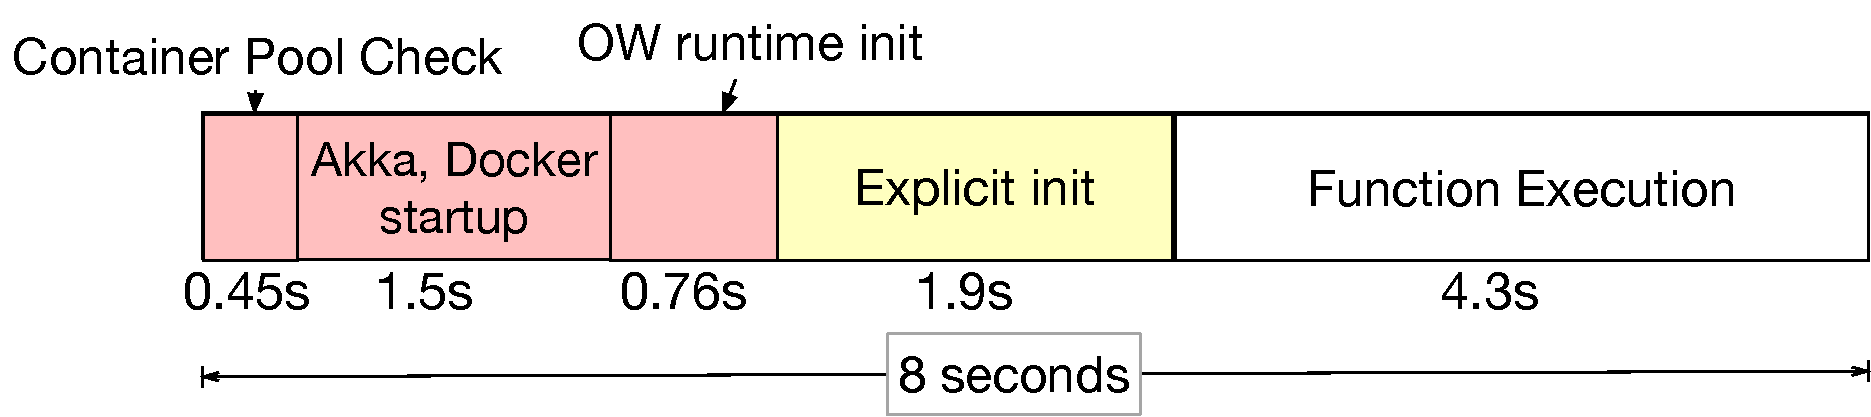
\includegraphics[width=0.47\textwidth]{../figures/ow-timeline.pdf}
  \vspace*{\myfigspace}
  \caption{Timeline of function execution and sources of cold start delay in OpenWhisk for an ML inference application.}
  \label{fig:timeline}
\end{figure}


\noindent \textbf{Function Initialization.}
%\noindent \textbf{Function Initialization.}
%
%Optionally, applications may also use custom code to initialize and pre-warm the container 
%rev1 first and last line 
%Explicit
Function initialization refers to function-specific code for downloading and resolving code and data dependencies, which can be run before actual function execution (explicit-init component in Figure~\ref{fig:timeline}). 
For example, this can be used for downloading data dependencies ahead of time such as large neural network models for inference, or for runtime initialization such as downloading and importing package dependencies (e.g., Python packages). 
%The second technique for reducing the cold start overhead is to explicitly initialize functions before running  them, and resolving most of the function's code and data dependencies during the initialization phase. 
%
An example of function initialization is shown in Figure~\ref{fig:lambda-example}, which shows a pseudo-code snippet of a function that performs machine learning inference on its input. 
For ML inference, the function downloads an ML model and initializes the TensorFlow ML framework (lines  5 and 6). 
If the function's container is kept alive, then invocations of the function do not need to run the expensive initialization code (lines 2--6). 
%Thus, the execution latency of functions can be minimized with a combination of careful function initialization and keeping the containers alive. 
% too broad a conclusion here...


% \footnotesize
\begin{figure}
\begin{lstlisting}[language=Python, numbers=left, frame=single, basicstyle=\footnotesize\sffamily, columns=fullflexible, xleftmargin=10.0ex, xrightmargin=10.0ex]
#Initialization code 
import numpy as np 
import tensorflow as tf
  
m = download_model('http://model_serve/img_classify.pb')
session = create_tensorflow_graph(m) 
  
def lambda_handler(event, context):
     #This is called on every function invocation 
     picture = event['data']
     prediction_output = run_inference_on_image(picture) 
     return prediction_output 
   \end{lstlisting}
   %\vspace*{\myfigspace}
   \caption{Initializing functions by importing and downloading code and data dependencies can reduce function latency by hiding the cold start overhead.}
   \label{fig:lambda-example}
   %\vspace*{\myfigspace}
\end{figure}


% The function cold start overhead includes both the execution environment initialization and the
\begin{comment}
Explicit initialization allows functions to be pre-warmed, and can be used to reduce the cold start overhead. 
However, explicit initialization is not common---our empirical investigation into FaaS benchmarks~\cite{kim_functionbench_2019} and official examples showed that applications do not use this functionality. 
Nevertheless, it can be a powerful technique to amortize expensive operations such as package imports and downloading data dependencies. 
Explicit initialization can thus increase the effectiveness of keep-alive. 
However because it is not ubiquitous, we assume it is \emph{optional}, and our keep-alive and provisioning techniques work with and without it. 
\end{comment}


\noindent \textbf{Workload Diversity and Dynamism.}
%
Designing keep-alive policies is not trivial due to the highly diverse and expanding range of applications that are using FaaS platforms.
%This is in tradeoffs category. 
Conventionally, FaaS has been used for hosting web services, which is attractive because of the pay-per-use properties. 
Event handling functions for web responses typically have a small memory footprint but require low execution latency. 
Increasingly, FaaS is also being used for ``heavy'' workloads with high memory footprint and large initialization overheads such as highly parallel numerical computing (such as matrix operations~\cite{jonas2017occupy}, scientific computing~\cite{shankar2018numpywren}, and machine learning~\cite{akkus_sand_2018}. 
The diversity of FaaS applications also results in a wide range of function memory footprints, running times, and initialization times, as seen in Table~\ref{tab:workloads}.  
Keep-alive policies must therefore balance the resource footprint of the containers with the benefits of keeping containers alive---and do so in manner that is applicable across a wide range of applications. 


Furthermore, FaaS workloads show a high degree of dynamism and temporal effects. 
The Azure function~\cite{shahrad_serverless_2020} trace shows sharp diurnal effects: the function arrival rate is about $2\times$ higher during the peak periods compared to the average. 
Function workloads are also heavy-tailed: a few ``heavy hitting'' functions are invoked much more frequently than others or consume a larger amount of computing resources, often by 2 or 3 orders of magnitude. 


\subsection{Policy Goals and Considerations}
\vspace*{\subsecspace}


The primary goal of keep-alive is to reduce the initialization and cold start latency, by keeping functions alive for different durations based on their characteristics. 
% Servers that run these functions are heavily multiplexed, and run hundreds of short lived functions concurrently. %backend FaaS servers?
% too sudden 
Because servers run hundreds of short lived functions concurrently, keep-alive policies must be generalizable and yield high server utilization. 
Functions can have vastly different characteristics, and keep-alive polices must work efficiently in highly dynamic and diverse settings. % (Table~\ref{tab:workloads}). 
We use the following characteristics of functions for keep-alive policies.


The \textbf{initialization time} of functions can vary based on the code and data dependencies of the function.  
For example, a function for machine learning inference may be initialized by importing large ML libraries (such as TensorFlow, etc.), and fetching the ML model, which can be hundreds of megabytes in size and take several seconds to download. 
Functions also differ in terms of their \textbf{total running time}, which includes the initialization time and the actual execution time. 
Again, functions for deep-learning inference can take several seconds, whereas functions for HTTP servers and microservices are extremely short-lived (few milliseconds). 
The \textbf{resource footprint} comprises of the CPU, memory, and I/O use, and also differs widely based on the application's requirements. 
Finally, functions have different \textbf{frequencies} and invocation rates. Some functions may be invoked several times a second, whereas other functions may only be invoked rarely (if they are used to serve a very low-traffic web-site, for instance). 

% \begin{figure}[t]
%   \centering
%   \vspace*{\myfigspace}
%   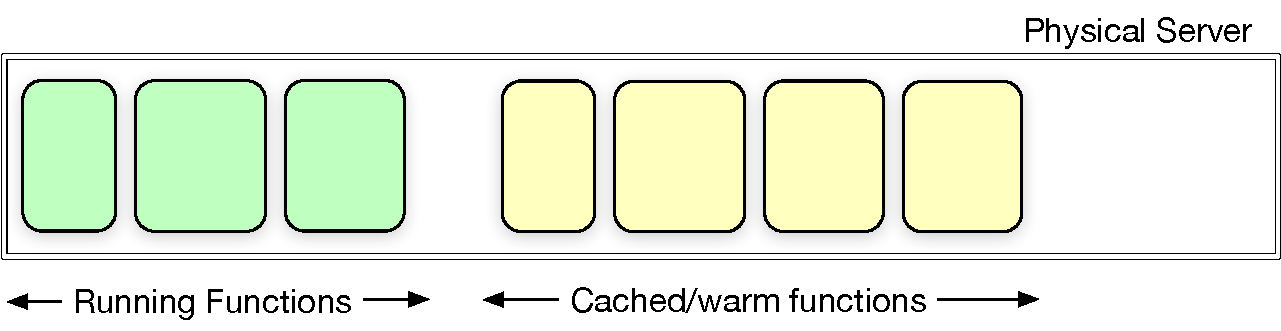
\includegraphics[width=0.4\textwidth]{../graphs/faas.pdf}
%   \vspace*{\myfigspace}
%   \label{fig:runwarm}
%   \caption{Server resources are consumed by running and warm containers.}
%     \vspace*{\myfigspace}
% \end{figure}


Because server resources are finite, it is important to prioritize functions which should be kept alive, based on the aforementioned characteristics. 
A function which is not popular and is unlikely to be called again in the near future, sees little benefits from keep-alive, and wastes server memory. 
%In fact, keeping such functions alive consumes valuable server computing resources for no gain in efficiency. %energy.. hmm
%Thus, keep-alive policies should prioritize popular functions. 
Similarly, the resource consumption of the functions is also important: since keeping large-footprint functions alive is more expensive than smaller functions, smaller functions should be preferred and kept alive for longer. 
Finally, functions can also be prioritized based on their initialization overhead, since it is effectively wasted computation.

% This paragraph is key. Different priorities and there is no one single ranking scheme for keepalive... 
The problem of designing keep-alive policies is complicated by the fact that functions may have vastly different keep-alive priorities for the different characteristics.
Consider a function with a large memory footprint (like those used in ML inference), high initialization overhead, and a low popularity.
Such a function should have a low keep-alive priority due to its size, high priority due to large initialization overhead, and a low priority due to its low popularity.
Thus, keep-alive policies must carefully balance all the different function characteristics and prioritize them in a coherent manner. 


% This still reads like making a case. But its only two sentences and bears repeating?
Current FaaS systems have shirked from this challenge and use primitive keep-alive policies that are not designed with the diversity and dynamism in mind. 
FaaS frameworks such as OpenWhisk, keep all functions alive for a \emph{constant} period of time (10 minutes). 
This is agnostic to different function characteristics such as resource footprint and initialization overheads, and only loosely captures popularity. 
More principled approaches are needed, which we provide next. 



%%% Local Variables:
%%% mode: latex
%%% TeX-master: "paper"
%%% End:


% Greedy dual policy

In this section, we discuss the system model for function keep-alive, the goals and considerations for keep-alive policies, and present our caching-inspired greedy-dual policy. 

\noindent \textbf{System model:} 
We assume that each function invocation runs in its own container. 
%
A FaaS platform may use a cluster of physical servers, and forward the function invocation requests to different servers based on some load-balancing policy. 
Our aim is to investigate general keep-alive techniques that are independent of the load-balancing, and we therefore focus on \emph{server-level} policies. 
Even on a single server, a function can have multiple independent and concurrent instantiations, and hence containers.
Each function has its own container image and initialization code, and thus containers cannot be used by multiple functions. 
A function's containers are nearly identical in their resource utilization, since they are typically running the same function code.
When a function finishes execution, its container may be terminated, or be kept alive and ``warm'' for any future invocations of the same function. 
%
At any instant of time, each container is either running a function, or is being kept alive/warm. % (see Figure~\ref{fig:server}). 
%
Thus, server resources are consumed by running containers, and containers being kept alive in anticipation for future invocations. 


%Before invoking a function, users need to register it with the FaaS platform.  
%Registering typically entails providing information about which language the function is written in, the function body, and any initialization code that the function execution requires. 


% Figure with running, cached, and free, can be referenced here? 
\vspace*{\subsecspace}
\subsection{Policy Goals and Considerations}
\vspace*{\subsecspace}

The primary goal of keep-alive is to reduce the initialization and cold-start latency, by keeping functions alive for different durations based on their characteristics. 
% Servers that run these functions are heavily multiplexed, and run hundreds of short lived functions concurrently. %backend FaaS servers?
% too sudden 
Because servers run hundreds of short lived functions concurrently, keep-alive policies must be generalizable and yield high server utilization. 
%
Functions can have vastly different characteristics, and keep-alive polices must work efficiently in highly dynamic and diverse settings. % (Table~\ref{tab:workloads}). 
We have identified the following characteristics of functions that are the most pertinent for keep-alive policies.


The \textbf{initialization time} of functions can vary based on the code and data dependencies of the function.  
For example, a function for machine learning inference may be initialized by importing large ML libraries (such as TensorFlow, etc.), and fetching the ML model, which can be hundreds of megabytes in size and take several seconds to download. 
Functions also differ in terms of their \textbf{total running time}, which includes the initialization time and the actual execution time. 
Again, functions for deep-learning inference can take several seconds, whereas functions for HTTP servers and microservices are extremely short-lived (few milliseconds). 
The \textbf{resource footprint} of functions comprises of their CPU, memory, and I/O use, and also differs widely based on the application's requirements. 
Finally, functions have different \textbf{popularities}, and are called with different rates. Some functions may be invoked several times a second, whereas other functions may only be invoked rarely (if they are used to serve a very low-traffic web-site, for instance). 

% \begin{figure}[t]
%   \centering
%   \vspace*{\myfigspace}
%   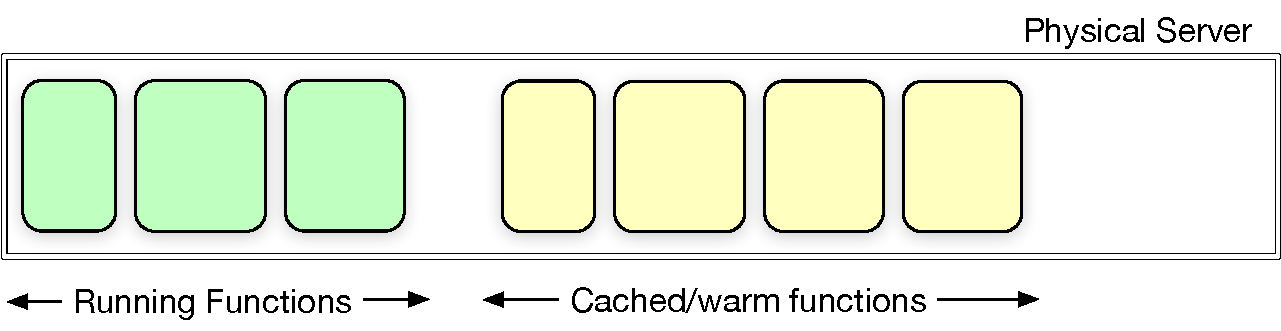
\includegraphics[width=0.4\textwidth]{../graphs/faas.pdf}
%   \vspace*{\myfigspace}
%   \label{fig:runwarm}
%   \caption{Server resources are consumed by running and warm containers.}
%     \vspace*{\myfigspace}
% \end{figure}


Because server resources are finite, it is important to prioritize functions that should be kept alive, based on the aforementioned characteristics. 
%
A function which is not popular and is unlikely to be called again in the near future, sees little benefits from keep-alive. 
In fact, keeping such functions alive consumes valuable server computing resources for no gain in efficiency. %energy.. hmm
Thus, keep-alive policies should prioritize popular functions. 
%
Similarly, the resource consumption of the functions is also important: since keeping large-footprint functions alive is more expensive than smaller functions, smaller functions should be preferred and kept alive for longer. 
%
Finally, functions can also be prioritized based on their initialization overhead, since it is effectively wasted computation.

% This paragraph is key. Different priorities and there is no one single ranking scheme for keepalive... 
The problem of designing keep-alive policies is complicated by the fact that functions may have vastly different keep-alive priorities for the different characteristics.
Consider a function with a large memory footprint (like those used in ML inference), high initialization overhead, and a low popularity.
Such a function should have a low priority due to its size, high priority due to large initialization overhead, and a low priority due to its low popularity.
Thus, keep-alive policies must carefully balance all the different function characteristics and prioritize them in a coherent manner.


FaaS frameworks such as OpenWhisk, keep all functions alive for a \emph{constant} period of time (30 minutes), or use LRU-based termination. 
%
These policies are agnostic to different function characteristics such as resource footprint and initialization overheads, and only loosely capture popularity. 
%
A more principled approach is needed, which we provide next. 


% \textbf{A small example should be described here with actual function characteristics and effect of const-TTL.}

% Thus, functions may have different keep-alive 

% Keep-alive policies can have a significant impact based on function characteristics, and have many different tradeoffs. 

% Since functions are executed 

% %Each of these functions have different characteristics, and smart keep-alive policies must run all 



% While keeping the containers alive can reduce the function execution latency, the running containers consume resources, which reduces the number of concurrent functions that can be executed. 

% We assume a single physical server runs many functions concurrently. 

% The number of functions that can be executed concurrently depends on the resource availability on the server.
% %
% Containers that are kept alive consume resources that can be used to run additional functions, and thus reduce the effective server utilization.

% Keep-alive thus imposes an important tradeoff. 
% %
% Policies must be cognizant of different factors.
% %
% The cold start (i.e., initilization) overhead, the total execution time, the resource footprint (i.e., memory occupied), and the frequency of the function invocation. 
% %

% Constant keep-alive policies (for 30 minutes) do not consider the resource footprints, nor do they take into account the benefits of warming for different functions.
% %
% For instance, given two containers close to their time out, we should ideally prefer the one with high cold-start overhead so that the work is not lost.

% Similarly, resource footprint is another major factor. Higher footprint containers should be evicted earlier.

% Ofcourse we need to consider multiple factors: footprint, access frequency, cold-start overhead, and size.
% %
% Optimizing for server-times 

% Our primary insight is that principled keep-alive policies can be derived if we look at this as a caching problem. 
% %
\vspace*{\subsecspace}
\subsection{Keep-alive is Equivalent to Caching}
\vspace*{\subsecspace}

Formulating a keep-alive policy that balances the characteristics of all competing functions, seems daunting. 
\emph{The central insight of this paper is that keeping functions alive is equivalent to keeping objects in a cache.} 


%The problem of what functions to keep alive and for how long, is equivalent to what objects to cache. 
Keeping a function alive reduces its effective execution latency, in the same way as caching an object reduces its access latency. 
When all server resources are fully utilized, the problem of which functions \emph{not} to keep alive is equivalent to which objects to \emph{evict} from the cache. 
The high-level goal in caching is to improve the distribution of object access times, which is analogous to our goal of reducing the effective function latencies. 


This caching analogy provides us a framework and tools for understanding the tradeoffs in keep-alive policies, and improving server utilization. 
%The problem of cache eviction in object caching is a thoroughly studied for a wide range of constraints, systems, and environments. 
Caching has been studied in wide range of contexts and many existing caching techniques can be applied and used for function keep-alive. 
Our insight is that we can use classic observations and results in object caching to formulate equivalent keep-alive policies, that can provide us with well-proven and sophisticated starting point for understanding and improving function keep-alive.  





% We assume that each function in its own container.
% When the function is ``registered'', this container image is created.
% Multiple concurrent invocations to the same function are possible, but each invocation is in its own container.
% Containers are in one of two states. Either running the function, or are idling when they are being kept warm. 
% When a function is called by the user, if a corresponding container is ``free'', then it is used to run the function.
% Otherwise, a new container is instantiated.

% When a container is launched, the initilization code runs.
% Depending on the application and the FaaS platform, the amount of initilization can be different.
% For example, a truly ``stateless'' function will include all required dependencies on every invocation.
% In any case, there is some initilization and start-up overhead, which consumes 


% While any caching/eviction algorithm can be used with the help of this analogy after the mapping, the algorithm must be cognizant of the different resource footprints and access frequencies and execution latencies of different functions.
% %
% The greedy dual approach is a good mapping, which we use below. 

\vspace*{\subsecspace}
\subsection{Greedy-Dual Keep-Alive Policy}
\vspace*{\subsecspace}

While many caching techniques can be applied to the function keep-alive policies, we now present one such caching-inspired policy that is simple and yet captures all function characteristics and their tradeoffs.
Our policy is based on Greedy-Dual-Size-Frequency object caching~\cite{gdsf}, which was designed for caches with objects of  different sizes, such as web-caches. 
Classical caching policies such as LRU or LFU do not consider object sizes, and thus cannot be completely mapped to the keep-alive problem where the resource footprint of functions is an important characteristic. 
As we shall show, the Greedy-Dual-Size-Frequency approach provides a general framework to design and implement keep-alive policies that are cognizant of the  frequency and recency of invocations of different functions, their initialization overheads, and sizes (resource footprints). 



Fundamentally, our keep-alive policy is a function \emph{termination} policy, just like caching focuses on eviction policies. 
%
Our policy is resource conserving: we keep the functions warm whenever possible, as long as there are available server resources.
%
This is a departure from current constant time-to-live policies implemented in public clouds, that are \emph{not} resource conserving, and may terminate functions even if resources are available to keep them alive for longer. 

%We assume that each functions is deployed in a container, and o
Our policy decides which container to terminate if a new container is to be launched and there is not enough resource availability.
%
The total number of containers (warm + running) is constrained by the total server physical resources (cpu and memory). 
%
Intuitively, our termination policy computes a ``priority'' for each container based on the cold-start overhead and resource footprint, and terminates the container with the lowest priority.
%
%Below, we describe our termination policy in detail.


%\noindent \textbf{Execution model.}
%Assume that there are $n$ different functions.
%
%We assume that each function runs in its own container.
%
%Each function can have multiple independent and concurrent instantiations, and hence containers. 
%
%At any instant of time, each container is either running a function, or is being kept alive/warm. 
%

%What is the point of this? 
%Assume that a  function $i$ has a initialization or startup time of $s_i$. 
%Once initialized, the running time of the function is  $r_i$, and thus total running time for the cold-start case is $s_i + r_i = T_i$.  
%When executing on a warm container, the time is simply $w_i$.
%


%Let $m_i$ be the memory footprint of the function.


%The total number of containers (warm + running) is constrained by the total server physical resources (cpu and memory). 
%Each container has a resource footprint, which we also call the \emph{size} of the container, denoted by $\mathbf{d_i}$.
%The size may be a multi-dimensional resource vector comprising of the CPU, memory, and I/O resources used by the running or warm container.
%In most scenarios, the number of containers that can run is limited by the physical memory availability, since CPUs can be multiplexed easily, and memory swapping can result in severe performance degradation.
%Thus for ease of exposition, we can consider only the container \emph{memory} use as the size, instead of a multi-dimensional vector. 


\noindent \textbf{Priority Calculation.} 
Our greedy dual policy is based on greedy dual caching~\cite{gdsf}. 
%
For each container, we assign a \emph{keep-alive priority}, which is computed based on the frequency of function invocation, its running time, and its size. 
%
The priority is given by:   \vspace*{-7pt}
\begin{equation}
  \vspace*{-7pt}
  \text{Priority} = \text{Clock} + \frac{\text{Freq} \times \text{Cost}} {\text{Size}}
    \label{eq:prio-prop}
\end{equation}
%
% 

On every function invocation, if a warm container for the function is available, it is used, and its frequency and priority are updated.
Reusing a warm container is thus a ``cache hit'', since we do not incur the initialization overhead. 
%
When a new container must be launched if there are insufficient resources, then containers are terminated based on their priority order---lower priority containers are terminated first. 
%
We now explain the intuition behind each parameter in the priority calculation:



\noindent \textbf{Clock} is used to capture the recency of execution.
%
We maintain a ``logical clock'' per server.
%
Each time a container is used, the server clock is assigned to the container and the priority is updated. 
%
Thus, containers that are not recently used will have smaller clock values (and hence priorities), and will be terminated before more recently used containers. 

The logical clock is updated only when a container is terminated. 
Containers are terminated only if there are insufficient resources to launch the new container and if existing warm containers cannot be used.  
%
Specifically, if a container  $j$ is terminated (because it has the lowest priority), then $\text{Clock} = \text{Priority}_j$.
All subsequent uses of other, non-terminated containers then use this clock value for their priority calculation.
%
In some cases, \emph{multiple} containers may need to be terminated to make room for new containers.
%
If $E$ is the set of these terminated containers, then $\text{Clock} = \max_{j \in E}{\text{Priority(j)}}$

We note that the priority computation is on a per-container basis, and containers of the same function share some of the attributes (such as size, frequency, and cost). 
However, the clock attribute is updated for each container individually.
This allows us to evict the oldest and least recently used container for a given function in order to break ties. 



\noindent \textbf{Frequency} is the number of times a given function is invoked.
%
A given function can be executed by multiple containers, and frequency denotes the \emph{total} number of function invocations across all of its containers. 
%
The frequency is set to zero when all the containers of a function are terminated.
%
The priority is proportional to the frequency, and thus more frequently executed functions are kept alive for longer. 
%
%This is a departure from object caching, where each object is distinct. In our case, because of concurrent executions of functions, multiple containers for the same function may exist, and we thus take into account all the 
%


\noindent \textbf{Cost} represents the termination-cost, which is equal to the initialization time, i.e., $s_i$. 
%
This captures the benefit of keeping a container alive and the cost of a cold-start. 
%
% There are other cost formulations also, such as $c/T$ etc that capture the ratio, that yield different policies.
The priority is thus proportional to the initialization overhead of the function. 





\noindent \textbf{Size} is the resource footprint of the container. 
%
%If we only care about the memory size, then we can simply use a single dimensional metric $m_i$ to denote the size.
%
The priority is inversely proportional to the size, and thus larger containers are terminated before smaller ones. 
%
We can use multi-dimensional resource vectors to represent the size, in which case we convert them to scalar representations by using the existing formulations from multi-dimensional \emph{bin-packing.}
%
For instance, if the container size is $\mathbf{d_i}$, then the size can be represented by the magnitude of the vector $||\mathbf{d_i}||$.
%
Other size representations can also be used.
A common technique is to normalize the container size by the physical server's total resources ($\mathbf{a}$), and then compute the size as $\sum_j \frac{d_j}{a_j}$ where $d_j, a_j$ are the container size and total resources of a given type (either CPU, memory, I/O) respectively.
%
Cosine similarity between $\mathbf{d}$ and $\mathbf{a}$ can also be used, as is widely used in multi-dimensional bin-packing. 

In most scenarios, the number of containers that can run is limited by the physical memory availability, since CPUs can be multiplexed easily, and memory swapping can result in severe performance degradation.
Thus for ease of exposition and practicality, we can consider only the container \emph{memory} use as the size, instead of a multi-dimensional vector. 



%


%







%%% Local Variables:
%%% mode: latex
%%% TeX-master: "paper"
%%% End:


\section{Server Provisioning Policies} % Resource provisioning ?
\label{sec:provision}

Resource provisioning, i.e., determining the size and capacity of the servers for handling FaaS workloads, is a fundamental problem in serverless computing. 
In this section, we develop techniques that allocate the appropriate amount of resources to servers based on the characteristics of the function workloads. 
Resource provisioning policies must consider the rate of function invocations, the resource footprints of the functions, and the inter-arrival time between function invocations. 
To handle the interplay and tradeoffs between these factors, we use similar principles for provisioning that we used for developing our keep-alive policies. 
% Previous three lines are a bit verbose and can be compressed to 2, but ok.. 
% rev 1 
In case FaaS workloads are co-located with other applications such as long-running containers and VMs, our provisioning policies can also be used to determine the resource allocation of the combined running and warm function pool. 

The fundamental challenge underlying resource provisioning for FaaS workloads is the performance vs. resource allocation tradeoff. 
Running a workload on large servers/VMs provides more resources for the keep-alive cache, which reduces the cold-starts and improves the application performance. 
However, we must also be careful to not \emph{overprovision}, since it leads to wasted and underutilized resources.
Additionally, since function workload can be dynamic, resource provisioning must be \emph{elastic}, and be able to dynamically scale up or down based on the load. 
We therefore present a \emph{static} provisioning policy that determines the server memory size for a given function workload, and then develop an elastic-scaling approach for handling workload temporal dynamics. 

\subsection{Static Provisioning}
\label{subsec:static}

In Section \ref{sec:bg}, we have seen how keeping function containers warm in a keep-alive cache can help mitigate the cold-start overheads. 
The effectiveness of any keep-alive policy depends on the size of this keep-alive cache, and thus the server resources available, i.e., the server size. 
Our \emph{static} provisioning policy thus selects a server size for handling a given workload. 
% Not peak, since that would be infinite sized. 90 percentile, but we dont do that. 
We want to optimize the resource provisioning to avoid over and under provisioning, both of which are detrimental to cost and performance respectively. 


Having established that keep-alive policies are equivalent to cache eviction in the previous section, we now extend the use of the caching analogy further, to develop a caching-based provisioning approach. 
We claim that the performance vs. resource availability tradeoff of serverless functions can be understood and modeled using cache hit (or miss) ratio curves.
%
Hit-ratio curves are widely used in cache provisioning and modeling, since they give insights into cache performance at different sizes. 
%The performance of caches is typically modeled by constructing a hit ratio curve, which determines the hit-ratio at different cache sizes.
%The ``optimum'' cache size is based on the marginal utility or the slope of the hit ratio curve. 
%Due to temporal locality of object references, hit-ratio curves are typically long-tailed, which makes provisioning... ? 
Once a hit-ratio curve is obtained, it is used to provision the cache size based on system requirements. 
A common approach is to size the cache based on a target hit-ratio (say, 90\%). 
Alternatively, the slope of a hit-ratio curve can be understood to be the marginal utility of the cache, and a cache size that maximizes this marginal utility is picked.
This entails choosing a cache size which corresponds to the \emph{inflection point} of the hit-ratio curve. 


% We use a similar approach.
\noindent \textbf{Hit-ratio Curve Construction.}
We use a function hit-ratio curve for determining the percentage of warm-starts at different server memory sizes. 
The hit-ratio curve is constructed by using the notion of \emph{re-use distances.}
A function's reuse-distance is defined as the total (memory) size of the unique functions invoked between successive invocations of the same function.
For example, in the request \emph{reuse} sequence of \texttt{ABCBCA}, the reuse distance of function \texttt{A} is equal to \texttt{size(B) + size(C)}.
%
The \emph{distribution} of these reuse distances can yield important insights into the required cache size.
If the cache size is greater than the reuse distances, then there will be no cache misses. 
This can be generalized to find the hit-ratio at cache size $c$:   \vspace*{-5pt}
\begin{equation}
  \label{eq:hrc-rdd}
  \text{Hit-ratio}(c) = \sum_{x=0}^cP(\text{Reuse-distance} = x),
    \vspace*{-5pt}
\end{equation}
where the reuse distance probability is obtained by scanning the entire input function workload for all reuse sequences. 
Conveniently, the hit-ratio is the CDF (cumulative distribution function) of the reuse distances, which can be empirically determined based on all the computed reuse distances. 
We show one such hit-ratio curve constructed with reuse distances, for a representative sample of the Azure function workload in Figure~\ref{fig:hrc}. 
We can see that the hit-ratio curve of functions \emph{also} follows the classic long-tailed behavior: the hit-ratio steeply increases with cache size up to an inflection point, after which we see diminishing returns. 


This technique and observation informs our provisioning policy.
We construct a hit-ratio curve based on reuse distances, and size the server's memory based on the inflection point.
Alternatively, we can set a target hit ratio (say, 90\%), and use that to determine the minimum memory size of the server. 
%
Finding the reuse-distances for an entire trace can be an expensive, one-time operation, and takes $O(N*M)$ time where N is the number of invocations and M is the number of unique functions. 
However, sampling techniques such as SHARDS~\cite{shards} can be applied to drastically reduce the overhead, making this a practical and principled technique for resource provisioning. 



\begin{figure}[t]
  \centering
  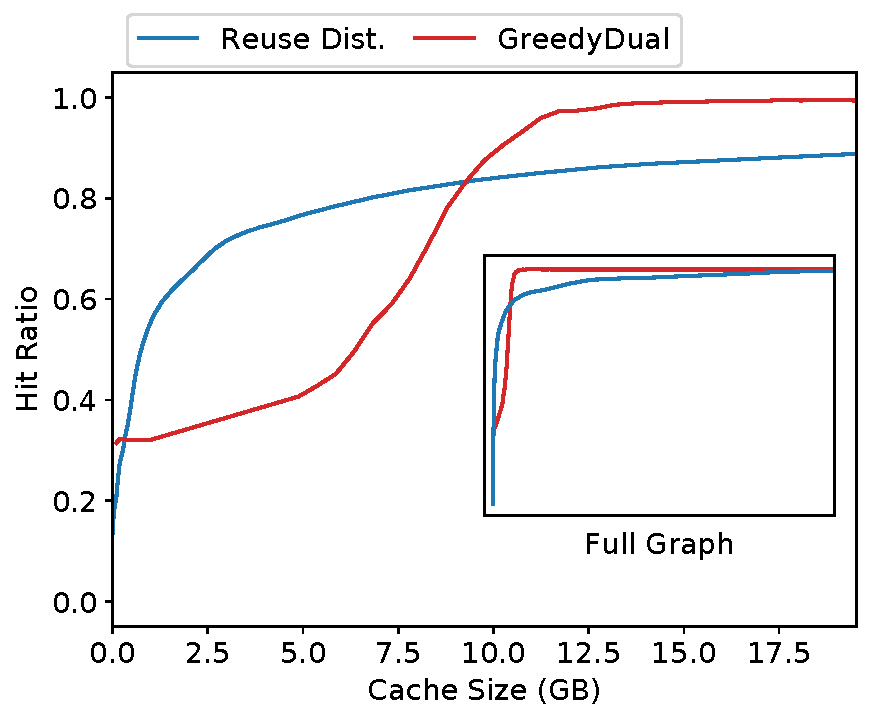
\includegraphics[width=0.5\textwidth]{faascache/faas-keepalive-20/graphs/rep-funcs-392/hit-ratio-392-b.pdf}
  \caption{Hit ratio curve using reuse distances show slight deviations from the observed hit ratios due to dropped requests at lower sizes, and concurrent executions at higher sizes.}
  \label{fig:hrc}
\end{figure}

\paragraph{Limitations of the Caching Analogy.}
The error in hit-ratios with the reuse-distance approach in Figure~\ref{fig:hrc} highlights an important facet where caching does not fully map to FaaS.
The main difference is due to the limitations on the concurrent execution of functions: 
caching deals with unique objects, whereas there can be  multiple containers for a function. 
%
At lower cache sizes, a high miss rate results in higher server load, and hence a higher number of dropped requests, that the classical reuse-distance approaches do not capture.
If all warmed containers of a function are in use, then a new invocation results in a cold-start---which would be counted as a cache ``hit''.
Thus at lower sizes, the real hit-ratio is lower than the ideal. 
At larger sizes, \emph{multiple} containers corresponding to concurrent invocations of a function will be present, which results in a deviation from the hit-rate curve. 
%: which is again different from the caching model where objects are unique. 
Reconciling these differences is an interesting area of future work. %but does not impact our work significantly. 
However, we note that hit-ratio curves are only used for coarse-grained allocation, and small deviations result in slight under or over provisioning. 
Moreover, our dynamic allocation policy described next can reduce these errors using proportional control. 

%\prat{Difference in two curves: could be because of multiple containers for a function, which is different from caching. So for larger cache sizes, the hit-ratio is higher. For lower sizes: it is lower because of dropped requests and not being able to handle the concurrent accesses which is not true with caching. So this is some sort of a negative result, or an area for future work.}


\subsection{Elastic Dynamic Scaling}
\label{subsec:dynamic}

We also use the hit-ratio curve approach for a \emph{dynamic} auto-scaling policy that adjusts the server size based on workload requirements. 
%
We assume that the FaaS server backend is running functions as containers either inside a virtual machine (VM), or is sharing the physical server with other cloud applications. 
In either case, it is important to be able to reclaim unused keep-alive cache resources and reduce its footprint, in order to increase the efficiency of the cloud platform. 

Our vertical elastic scaling policy is simple and is intended to demonstrate the efficacy of a general caching based approach. 
We implement a  proportional controller~\cite{pid-wiki} which periodically adjusts the VM memory size based on the rate of cold-starts.  
Thus during periods of low rate of function invocations (i.e., arrival rate), the cache size can be reduced. 
This may \emph{increase} the miss-ratio---but we care about the cold-starts (i.e., misses) per second, which is product of miss-ratio and invocations per second.
Our controller monitors the arrival and cold-start rate, and uses the hit-ratio curve to decrease or increase VM size dynamically. 
We use VM resource deflation~\cite{deflation-eurosys19} to shrink or expand the VM by using a combination of hypervisor level page swapping, or guest-OS memory hot-plug and unplug. 


Assume that we have a target miss speed (number of cold-starts/misses per second).
For instance, this target value can be a product of the desired hit-ratio, $h$, and the average function arrival rate for the entire workload trace, $\bar{\lambda}$. 
Periodically, we monitor the exponentially smoothed arrival rate $\lambda$, and the observed miss speed.
Our proportional controller adjusts the cache size in order to reduce the difference between the actual vs. target miss speed.
This error is used to compute the new \emph{miss rate}, $m$, and the associated cache size $c'$ as follows:
\begin{align}
  \label{eq:dyn}
%  m & = \frac{\bar{\lambda}}{\lambda}*h \\
  \text{HR}(c') & = 1-m = 1 - h\frac{\bar{\lambda}}{\lambda}
\end{align}

\noindent The new cache size $c'$ is then determined by inverting the hit-rate function $\text{HR}$.
Our vertical scaling controller is designed for coarse-grained VM size adjustments, and only tracks the workload at time granularities of several minutes. 
Our intent with this policy is to not be overly aggressive with the capacity changes, but only to capture the coarse diurnal effects. 
Therefore, we use a large error deadband: the cache size is only updated if the error is more than 30\%. 
%More sophisticated, predictive and reactive auto-scaling policies from web-clusters~\cite{gandhi2012autoscale} can be also be adapted. 
Finally, the memory scaling can also be combined with cpu auto-scaling based on the function arrival rate, using classical predictive and reactive auto-scaling techniques found in web-clusters~\cite{gandhi2012autoscale}. 

\paragraph{Online adjustments.} %rev1
Our policies rely on the \emph{aggregate} function characteristics, which is used for constructing the hit-ratio curve. 
Once done, the traffic intensity (invocations per second) can change.
We primarily assume that the probability distribution of function characteristics such as their frequency and size, does not significantly change.
However, our dynamic scaling policy can adjust to changes in the traffic intensity (invocations per second). 
In other words, we assume that the future traffic is going to be similar to the past, which is the basis of the timeseries-forecasting based policies (such as in ~\cite{shahrad_serverless_2020}), and is the fundamental principle underlying caching in general. 
%
Our provisioning policies are not completely online, since they have a preparation phase for constructing the hit-rate curves. 
A ``drift'' in function characteristics is fixed by periodically updating the hit-ratio curve, which we currently do once per week. 
Online hit-ratio curves can also be constructed, and adapting techniques such as ~\cite{zhang2020osca} is part of our future work.





% Let the exponentially smoothed arrival rate of functions be $\lambda$. 

% The hit-ratio curve constructed for the static provisioning is applicable for the overall workload for the average arrival rate $\bar{\lambda}$.
% For the elastic scaling, we monitor the exponentially smoothed arrival rate, $EWMA(\lambda)$, and scale up or down if it is more than one standard deviation from $\bar{\lambda}$. 
% If $\lambda < \bar{\lambda}$, we scale the server's memory down by $\delta(m)$, which is determined based on the cache hit ratio curve to meet the average or the set number of misses per second. 


% Let current cache size be c, and load be $\lambda$.
% In general, the misses per second is given by $m = (1-HR(c))\lambda$.
% The goal is to keep this constant, that is $m = \bar{m}$.
% If the new cache size is $c'$, then we have: $(1-HR(c'))\lambda  = (1-HR(c))\bar{\lambda}$
% \begin{equation}
%   \label{eq:dyn} 
%   HR(c') = 1- \dfrac{(1-HR(c))\bar{\lambda}}{\lambda} 
% \end{equation}
% We use the hit-rate curve to thus find $c'$ that yields the hit-rate on the right hand side of the above equation.  

% tgt-miss-rate = avg-lambda/lambda*miss-ratio 


%%% Local Variables:
%%% mode: latex
%%% TeX-master: "paper"
%%% End:


\section{Implementation}
\vspace*{\subsecspace}
\section{Implementation}

We have implemented the keep-alive and the provisioning policies as part of our FaasCache framework built on top of OpenWhisk (Figure~\ref{fig:sys}). 

\begin{figure}[t]
  \centering
  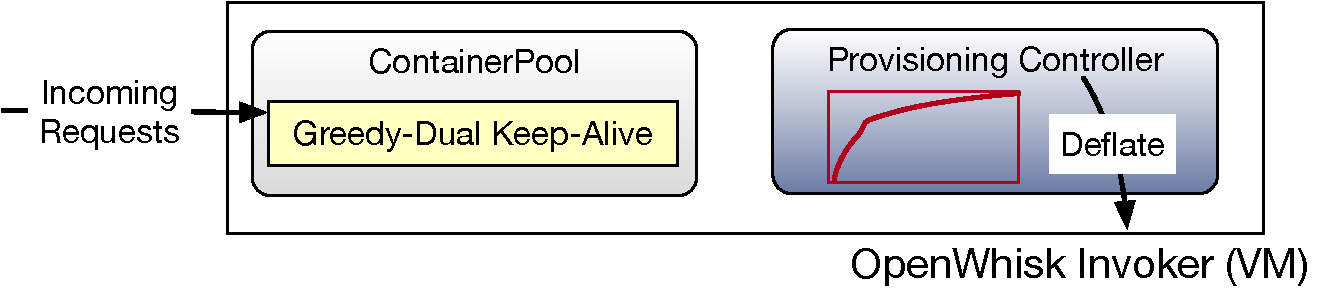
\includegraphics[width=0.95\textwidth]{faascache/faas-keepalive-20/figures/faascache.pdf}
  \caption{FaasCache system components. We build on OpenWhisk and augment it with new keep-alive policies and a provisioning controller. }
  \label{fig:sys}
\end{figure}

\noindent \textbf{Keep-Alive.}
FaasCache replaces the default OpenWhisk TTL-based keep-alive policy with the Greedy-Dual-Size-Frequency approach. 
For each initialized container, we assign and maintain the keep-alive prioritized ContainerPool, which is only a 100-line Scala modification. 
%Initialized containers are managed by the ContainerPool.
%\emph{Interesting aspects of priority calculation?} How is size, clock, frequency, cost, etc. computed? How does the impl differ from the idealized description? 
Each invocation of a function (OpenWhisk action) in ContainerPool records the launch time and when results are returned.


If the container was prewarmed before the invocation arrived, we record it as the function's warm runtime.
For new functions, the initialization overhead is captured and assumed to be the worst-case runtime until a warmed invocation is recorded. % is approximated as the minimum overhead of Docker and OpenWhisk's Python runtime initialization.
In the subsequent invocations, the initialization overhead is computed by subtracting the cold from the warm time. 
%Otherwise it was a cold start.
%The maximum cold and warm runtimes are kept per function to compute the priority.
%Size is simply the number of megabytes of memory OpenWhisk preallocates to the action's container, and
The function's frequency and clock value are updated with each request.
If the last container of a function is evicted, its cold and warm runtimes are stored and used to compute priority for its future invocations. 
%
To preserve the invocation fast-path, the ContainerPool is not kept sorted by priority. 
%Priorities are computed when an eviction needs to be made to reclaim memory.
Instead, it is sorted by priorities only during evictions, when the lowest priority container(s) are terminated.
%
We batch eviction operations to optimize the slow-path: we evict multiple containers to reach a certain free resource threshold (1000 MB is the current default). 

%rev 1
In the future, we intend to implement a similar design that is found in the Linux kernel page eviction. A separate thread (analogous to kswapd) can be used to periodically sort the containerpool list and asynchronously evict containers, so that eviction is not on the critical path. 

%All of an action's containers share one priority, regardless of the last time each ran an invocation.

% \prat{How are the values inferred?}
% New functions always replace old functions in the ContainerPool, so the priority of newly inserted containers doesn't matter. 
% After the second invocation of a function, its initialization overhead is inferred as the difference between the cold (first) and warm (subsequent) invocations. 
% Memory usage of the container is gathered via {\em Docker stats?\/}.



\noindent \textbf{Provisioning.}
For the static provisioning, we compute the reuse distance distribution for a given workload trace, and assume stationarity --- that it will be applicable on similar future workloads. 
We compute the reuse distances conventionally, by examining all reuse-sequences.
The dynamic provisioning controller runs periodically (every 10 minutes), to deflate or inflate the VM size, if the cold start rate deviates from the target significantly (by more than 30\%).
When the VM has to be shrunk, we use cascade deflation~\cite{deflation-eurosys19}.
We shrink the ContainerPool first, and reclaim the free memory using guest OS-level memory hot-unplug and hypervisor-level page swapping. 
%This approach is based on cascade deflation proposed in~\cite{deflation-eurosys19}. 

%Optimizations such as SHARDS that can significantly reduce the running time by sampling a small fraction of the functions, were found to be inadequate due to the wide disparity in the function sizes.
%The efficacy of sampling based techniques like SHARDS has mainly been empirically established only for fixed-sized objects. 


\noindent \textbf{Keep-alive Simulator.}
We have implemented a trace-driven discrete event simulator for implementing and validating different keep-alive policies.
Our simulator is written in Python in about 2,000 lines of code, and implements the various variants described in Section~\ref{subsec:variants}. 
It allows us to determine the cache hit ratios and the cold start overheads for different workloads and memory sizes.
Additionally, it also implements the static and dynamic provisioning policies for adjusting server size.

%%% Local Variables:
%%% mode: latex
%%% TeX-master: "paper"
%%% End:


%\vspace*{\subsecspace}
\section{Experimental Evaluation}
%\vspace*{\subsecspace}
\section{Experimental Evaluation}

% section Evaluation
\label{sec:eval}


We now present the experimental evaluation of our caching-based keep-alive technique by using function workload traces and serverless benchmarks.
Our goal is to investigate the effectiveness of these techniques under different workload and system conditions. 


\begin{figure*}
  \centering
\subfloat[ Representative functions.     \label{fig:rep-trace-exec}]
{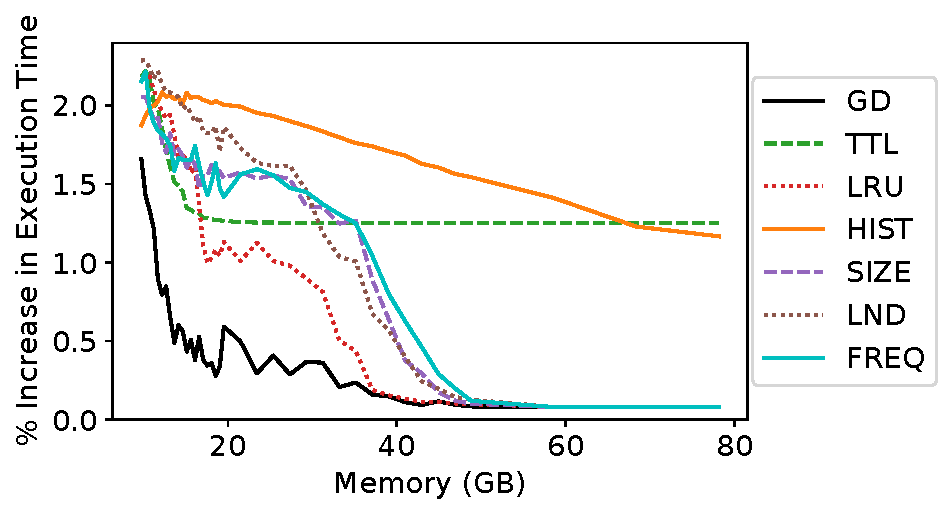
\includegraphics[width=0.37\textwidth]{faascache/faas-keepalive-20/graphs/rep-funcs-392/exec_inc_mem-392-legend.pdf}}
  \hfill 
    \subfloat[Rare functions.     \label{fig:rare-trace-exec}]
{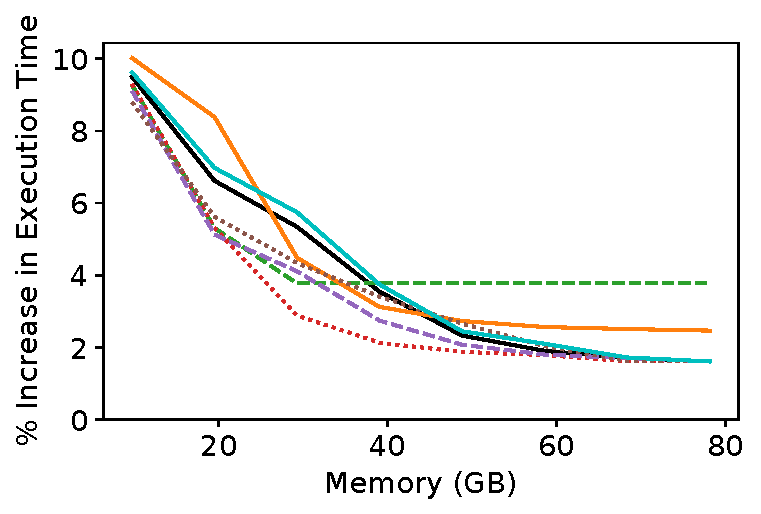
\includegraphics[width=0.3\textwidth]{faascache/faas-keepalive-20/graphs/rare-funcs-1000/exec_inc_mem-1000.pdf}}
\hfill 
  \subfloat[Random sampling.      \label{fig:random-trace-exec}] {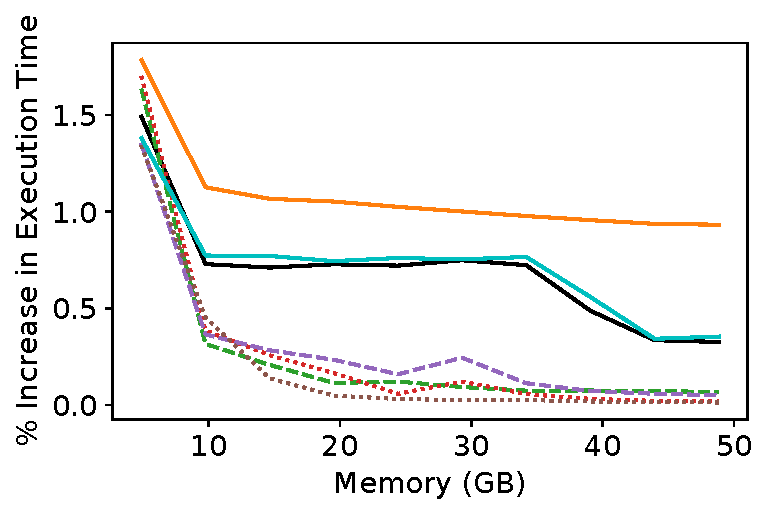
\includegraphics[width=0.3\textwidth]{faascache/faas-keepalive-20/graphs/random-funcs-200/exec_inc_mem-200.pdf}}
\caption{Increase in execution time due to cold starts for different workloads derived from the Azure function trace.}
\label{fig:exec-overheads-all}
\end{figure*}


\begin{figure*}[t]
  \centering
%  \vspace*{\myfigspace}
%  \begin{minipage}[c]{0.7\linewidth}
  \subfloat[Representative functions.\label{fig:rep-trace-cold}] {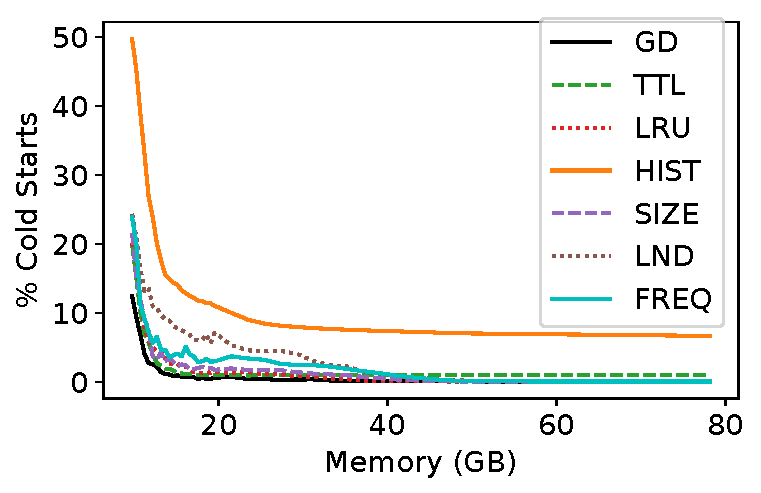
\includegraphics[width=0.33\textwidth]{faascache/faas-keepalive-20/graphs/rep-funcs-392/cold_drop_mem-392-legend.pdf}}
  \hfill
    \subfloat[Rare functions. \label{fig:rare-trace-cold}] {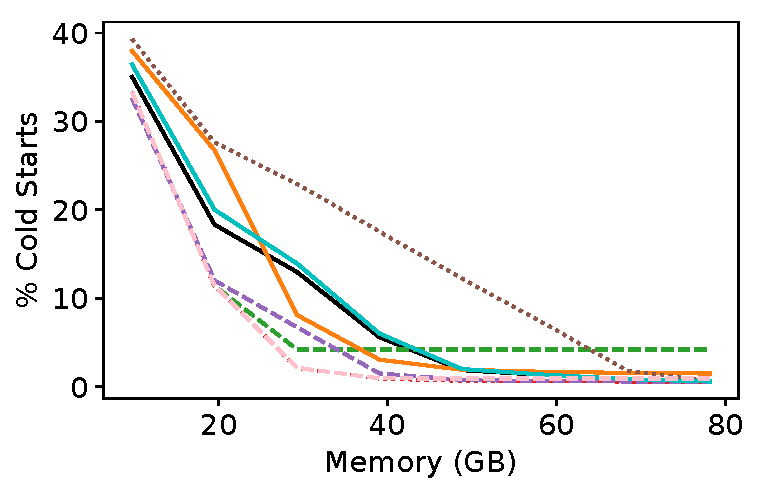
\includegraphics[width=0.33\textwidth]{faascache/faas-keepalive-20/graphs/rare-funcs-1000/cold_drop_mem-1000.pdf}}
  \hfill
  \subfloat[Random sampling. \label{fig:random-trace-cold}]
  {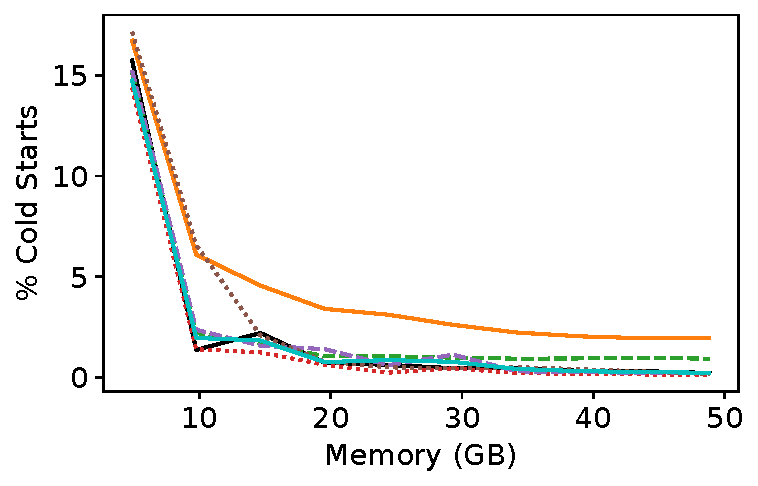
\includegraphics[width=0.33\textwidth]{faascache/faas-keepalive-20/graphs/random-funcs-200/cold_drop_mem-200.pdf}}
    \caption{Fraction of cold starts is lower with caching-based keep-alive. } % for different samples of the Azure function trace.}
      \label{fig:cold starts-all}
%    \end{minipage}
%    \hfill
%    \begin{minipage}[c]{0.29\linewidth}
 %      \begin{figure}
 %     \end{figure}
%    \end{minipage}
\end{figure*}


%%%%%%%%%%%%%%%%%%%%%%%%%%%%%%%%%%%%%%%%%%%%%%%%%%%%%%%%%%%%
\noindent \textbf{Setup, Workloads, and Metrics.}
%
For evaluating different keep-alive performance with different workload types, we use different trace samples from the Azure Function trace~\cite{shahrad_serverless_2020}, which contains execution times, memory sizes, and invocation-timestamps for more than 50,000 unique functions. 
Since our goal is to examine performance at a \emph{server} level, we use smaller samples of this trace for realistic server sizes, and replay them in our discrete-event keep-alive simulator. 
This also allows us to examine the behavior with different \emph{types} of workloads, which is important because our keep-alive policies are designed to be general and workload-agnostic.
We use the following three trace samples (more details in the Table~\ref{tab:trace-deets}): \\
\noindent \textbf{RARE:} A random sample of 1000 of the rarest, most infrequently invoked functions. These functions will usually result in cold starts under a classic 10 minute TTL.  \\
% mention 75% percentile detail?
\noindent \textbf{REPRESENTATIVE:} A sample of 400 functions, sampled from each quartile of the dataset based on frequency---yielding a more representative sample with higher function diversity. \\
\noindent \textbf{RANDOM:} A random sample of 200 functions.

% The FaasCache system is evaluated in Section~\ref{subsec:ow-eval}.
Functions from the FunctionBench~\cite{kim_functionbench_2019} suite are used for generating a realistic workload. 
A single server with 250 GB RAM and 48-core Intel Xeon Platinum 2.10 GHz CPUs is used for running all functions. The server is running modified OpenWhisk (i.e., FaasCache), and Ubuntu 16.04.5. 

\begin{table}
  \centering
  \caption{Size and inter-arrival time (IAT) details for the Azure Function workloads used in our evaluation.}
  \begin{tabular}{lrrr}
    \hline 
    Trace & Num Invocations & Reqs per sec & Avg. IAT \\
    \hline
    Representative & 1,348,162 & 190 /s & 5.4 ms \\
    Rare & 202,121 & 30 /s & 36 ms \\
    Random & 4,291,250 & 600 /s & 1.8 ms \\
    \hline
  \end{tabular}
  \label{tab:trace-deets}
\end{table}



\paragraph{Adapting the Azure Functions Trace.}
The format of the original Azure Function trace~\cite{shahrad_serverless_2020} requires some additional pre-processing and extrapolation for generating a workload.  
The full dataset consists of 14 days of function invocations, and billions of individual invocations. We use the first day's data, and do not consider functions that are never reused (i.e., with less than two invocations). 

The original trace provides memory consumption at the \textit{application} level---with the application made up of multiple functions.
Therefore, we evenly split the memory allocation between all functions in an application.
The dataset provides invocations in minute-wide buckets.
When injecting/replaying the workload, if there is only one invocation in a minute-bucket, it is injected at the beginning of the minute. 
For multiple invocations, they are equally spaced throughout the minute. 

%
The cold start overhead of each function is estimated as {\texttt maximum - average} runtime, and the execution times provided in the dataset are used for this computation. 
The dataset does not account for certain important sources of cold start overheads such as execution environment creation (e.g., Docker).
This unfortunately underestimates the cold start overheads.
However, because it applies uniformly to all functions, it preserves the relative performance of the different keep-alive policies, and does not affect the cache hit ratios. 
%

%These cold start overheads are generally constant, 

%This may not capture all the sources of cold start overhead such as the execution environment creation (e.g., Docker) and 

We are interested in two metrics: the cold start ratio; and the average increase in the execution time due to cold starts.
The increase in execution time is computed by averaging across all function invocations. 

%The latter captures the heterogeneity in function initialization overheads and invocation frequencies. 
%For estimating the time each function spends in explicit initialization, using the workload trace we subtract each functions' average runtime from its maximum runtime. 
%The dataset timings do not include provider overhead, so this initialization time is entirely due to application code.

%%
%Provider cold start overheads can be up to several seconds long, and take up the plurality of a function's execution time.
%Because the dataset does not include provider overhead, it is impossible to assign a realistic number to this cost.
%With these large penalties are not in our simulations, we therefore assume it as 0, but in reality the overhead is roughly constant.
%This causes the global increase in execution time to be smaller than it would be otherwise.
%Including a non-zero cold start cost would apply uniformly across all functions, and thus not change eviction priorities relative to one another.
%The cache hit ratio in Figure~\ref{fig:cold starts-all} would remain unchanged, and the Y-axis (the global increase in execution time) of Figure~\ref{fig:exec-overheads-all} would be scaled up relative to the chosen cold start overhead.
%%

% Using variable, real-world, times would require knowing or randomly assigning the runtime of functions, and would still require stochasticity as provider latency is not constant. 

% Not explaining this in the paper was our biggest “oops”: and there’s a few sources of confusion.
% Here is what we assumed: the dataset doesnt include container startup time, but the included function execution time captures both the function-initialization time (importing packages etc.), and the actual execution.
% So the assumption is that the Max execution time was due to this initialization overhead (which we include in the cold start overhead in our paper).
% The “time functions take to execute after they are ready to run” added to our confusion: we assumed this meant that it is the time when the control is transferred to the FaaS runtime inside the container: which would still incorporate all actual function initialization overheads.
% A contributing factor to making this assumptions was that most OpenWhisk applications do not have a strict explicit initialization, so it is in general not possible to know when a function is truly ready to execute non-idempotent code. 

% And so we end up with pretty small startup overheads, which can be seen from our Figure 5.
% Including container startup time and other overheads would make little difference to relative performance, since the extra overhead would apply to all functions.
% For instance, adding a constant startup penalty for all functions doesnt change their eviction priorities.
% The cache hit ratio (our Figure~\ref{fig:cold starts-all}) would remain unchanged, and the Y-axis of Figure~\ref{fig:exec-overheads-all} would be scaled up depending on the chosen cold start overheads. 

\begin{comment}
Our simulator evaluation uses real-world FaaS usage data from the recently released Azure Function trace~\cite{shahrad_serverless_2020}. 
The entire trace consists of tens of thousands of functions with billions of invocations, making it intractable to simulate the entire dataset.
Trace sampling methodology is important to capture the characteristics of the overall trace, and the scenarios where FaasCache is most effective.
Over half of all functions have an interval arrival time (IAT) over 30 minutes, where IAT is defined as execution time + idle time, guaranteeing them to always have cold starts when using a simple TTL eviction policy.
A tiny 1\% of functions account for nearly 90\% of all invocations, with an IAT of under a minute. 
% Therefore, smaller samples 
Given these extreme disparities, smaller samples must match behaviors of the larger dataset to show their effectiveness.
The full Azure trace can be suitably handled by a cluster of servers, in which case the system behavior is influenced by load-balancing and sharding policies, which our work is orthogonal to.
%Explain the rationale here. 
We generate three day-long traces using the Azure Functions dataset to showcase the effectiveness of FaasCache.
\prat{Insert reuse distance vs. time heatmaps for all these traces in the appendix along with table describing: number of fns, total invocations, avg. inter arrival time, etc.}
\end{comment}

%%%%%%%%%%%%%%%%%%%%%%%%%%%%%%%%%%%%%%%%%%%%%%%%%%%%%%%%%%%%
\subsection{Trace-Driven Keep-Alive Evaluation}

In this subsection, we use the Azure function traces to evaluate different keep-alive policies in our discrete-event simulator. 
% Primary Comparison? Competitors? 
We compare all caching-based variants against the default keep-alive policy in OpenWhisk (10 minute TTL).
% rev 1
When the server is full, this TTL policy evicts containers in an LRU order.
We also evaluate different Greedy-Dual variants: GD is our GDSF policy described in Section~\ref{subsec:gdsf}.
The others are the caching-based variants described in Section~\ref{subsec:variants}: LND is Landlord, and FREQ is LFU. 


%rev 1 
We also compare against the histogram-based keep-alive policy in~\cite{shahrad_serverless_2020}, which is the state of the art technique.
% Section 4.2 of serverless paper 
We have reproduced this policy (HIST) from the details in the paper, and have implemented it in a ``best-effort'' manner without any knowledge of the optimizations in the actual implementation.
This is effectively a ``TTL+Prefetching'' policy: it uses a histogram of \emph{inter-arrival times} to predict future function invocations and eagerly evict warm functions.
It uses timeseries forecasting to capture temporal locality, but does not consider the other function characteristics such as function size and initialization cost. 
The IAT, computed by taking a function's execution time plus the subsequent idle time, between each actual invocation is recorded in minute granularity buckets, tracking up to four hours between executions.
The policy uses ARIMA modeling for those invocations that fall outside this four hour window, we chose not to implement this specific feature due to its complexity, and the fact that it accounted for a minor fraction (\textasciitilde 0.56\%) of all invocations.
From these buckets, a function's coefficient of variation (CoV) is calculated using Welford's online algorithm~\cite{welford}. 
When the function's IAT is predictable (CoV $\leq 2$), the function's historical/customized preload and TTL time are used.
Otherwise, the function has a generic TTL of two hours. 
When an invocation is anticipated, it is brought into memory and kept there until its TTL expires.
A function is evicted when the policy predicts it will not have an invocation in the near future. 
%We chose not to implement the ARIMA modeling for IAT's exceeding four hours for simplicity and the fact it is only applicable to a tiny number of functions.
% \textbf{More details. Histogram size? When created? Online? }


%
The increase in execution time for different traces and for different cache sizes is shown in Figure~\ref{fig:exec-overheads-all}.
% How is this measured?
The increase in execution time is the cold start overheads averaged across all invocations of every function, and captures the user-visible response-time. 
%

For the representative trace (Figure~\ref{fig:rep-trace-exec}), Greedy-Dual reduces the cold start overhead by more than $3\times$ compared to TTL for a wide range of cache sizes (15--80 GB). 
Interestingly, it is able to achieve a low overhead of only 0.5\% at a much smaller cache size of 15GB, compared to other variants, which need 50 GB to achieve similar results---a reduction of cache size by more than $3\times$. 
%
For rare functions (Figure~\ref{fig:rare-trace-exec}), caching-based approaches such as LRU  reduce the cold start overhead by $2\times$ compared to TTL for cache sizes of 40--50 GB. 
This shows that for rare functions, recency is a more pertinent characteristic, and the complex four-way tradeoff used in Greedy-Dual is not necessarily ideal in all workload scenarios. 
For this workload, the HIST policy outperforms TTL, as reported in~\cite{shahrad_serverless_2020}. 
However, it results in 50\% higher cold start overhead compared to caching-based approaches.
Furthermore, because HIST uses only inter-arrival times, it is unable to perform well with heterogeneous representative workloads  (Figure~\ref{fig:rep-trace-exec}). 


Finally, the randomly sampled trace has a large number of infrequent functions because of the low probability of selecting the heavy-hitting functions.
In Figure~\ref{fig:random-trace-exec}, the recency component again dominates, and we see LRU outperforming other variants. 
The equivalence of LRU and TTL-based caching for rare objects has been noted~\cite{basu2017adaptive,jiang2018convergence}, which explains their similar behavior seen in Figure~\ref{fig:random-trace-exec}. 
%closeness of TTL and LRU performance for rare functions in our result. 


\noindent \emph{\textbf{Result:} For representative, diverse workloads, our GD policy can improve the performance and shrink cache sizes by up to $3\times$. For more homogeneous workloads, LRU can outperform current TTL-based approaches by $2\times$.}

%%%
% rev 1 
We can observe from Figure~\ref{fig:exec-overheads-all} that the increase in execution time is generally small ($<10\%$).
This is because of two main factors: the evaluation metric chosen, and the properties of the workload trace. 
The execution time is averaged across \emph{all} function invocations.
However, serverless workloads consist of a large number of very frequently invoked functions. 
The performance of these functions is generally not affected by keep-alive policies, since any policy is going to keep them in the cache because of their high frequency. 
Thus, the difference between non-work-conserving policies such as TTL and Greedy-Dual is masked because of the frequent and popular functions. 
For instance, the average inter-arrival time for all three workloads is less than 36ms, or about 27 function invocations per second. 
Thus, the server is overloaded, and TTL does well even though it is not work-conserving. 
As the IAT grows, the effectiveness of work-conserving caching-based approaches increases compared to TTL, as we shall see in the next subsection. 

%%%%
%While Figure~\ref{fig:exec-overheads-all} focuses on the average increase in execution latency, keep-alive can also reduce the tail latency of functions. Cold start 

%%%%

We see a similar relation and behavior in the miss-ratio curves shown in Figure~\ref{fig:cold starts-all}. 
Due to function heterogeneity, the cold start overheads are not strictly correlated with cache miss ratios, and thus the differences between policies is different compared to the previously described actual cold start overheads. 
% \prat{Write after colors are fixed.}
Classic miss-ratio curves do not consider the miss \emph{cost} (i.e., initialization cost), which is an important metric that is optimized by the Greedy-Dual approach.
Thus, in general, even in object caching contexts, miss-ratio curves deviate from the actual performance---a behavior that we also observe. 

%%%%%%%%%%%%%%%%%%%%%%%%%%%%%%%%%%%%%%%%%%%%%%%%%%%%%%%%%%%%
\subsection{OpenWhisk Evaluation}
\label{subsec:ow-eval}



\begin{figure}
  \centering
  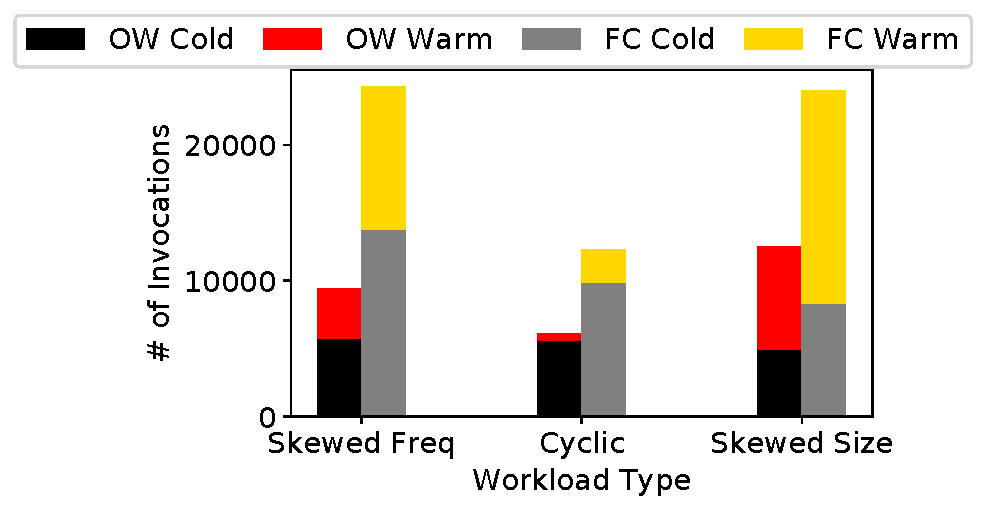
\includegraphics[width=0.6\textwidth]{faascache/faas-keepalive-20/graphs/litmus_tests/litmus_2_stacked.pdf}
  \caption{FaasCache runs 50 to 100\% more cold and warm functions, for skewed workload traces.}
  \label{fig:litmus_2}  
\end{figure}


In this subsection, we evaluate the performance of the FaasCache system on real functions. 
We focus on the performance of FaasCache's Greedy-Dual keep-alive implementation, and compare it to the vanilla OpenWhisk system which uses a 10 minute TTL.


% rev1 1
In contrast to the previous subsection in which we showed the average performance for different cache sizes, we will now also focus on the inverse problem: for a fixed server size, how much more load can be handled with FaasCache? 
By leveraging Greedy-Dual caching, FaasCache is able to reduce cold starts. 
This also reduces the number of \emph{dropped} requests. %

OpenWhisk buffers and eventually drops requests if it cannot fulfill them.
Because FaasCache more effectively selects evictions, its higher hit rate results in functions finishing faster, allowing more functions to be executed in the same time frame.  
%
\begin{table}
  \centering
  \caption{FaaS workloads are highly diverse in their resource requirements and running times. The initialization time can be significant and is the cause of the cold start overheads, and depends on the size of code and data dependencies.}
  \begin{tabular}{lrrr}
    \hline 
    Application & Mem size & Run time & Init. time \\
    \hline
    ML Inference (CNN) & 512 MB & 6.5 s & 4.5 s \\
    Video Encoding & 500 MB & 56 s & 3 s \\
    Matrix Multiply & 256 MB & 2.5 s & 2.2 s \\
    Disk-bench (\texttt{dd})  & 256 MB & 2.2 s & 1.8 s \\
    Image Manip & 300 MB & 9 s & 6 s \\
    Web-serving & 64 MB & 2.4 s & 2 s \\
    Floating Point & 128 MB & 2 s & 1.7 s \\
    \hline
  \end{tabular}
  % \vspace*{\myfigspace}
  \label{tab:fc:workloads}
  %\vspace*{\myfigspace}
\end{table}

To examine the effect of Greedy-Dual keep-alive on cold start and dropped requests, we use a workload trace comprising of four different functions: Disk-bench, ML inference, Web-serving, and Floating-point, described in Table~\ref{tab:fc:workloads}.

In Figure~\ref{fig:litmus_2}, we use different kinds of \emph{skewed} workloads: with a single function having a different frequency, a cyclic access pattern, and a skewed workload with 2 sizes. 
We see that FaasCache's keep-alive can increase the number of warm invocations by between 50 to 100\% compared to OpenWhisk's TTL.
The difference in the total number of requests served (warm+cold) is because OpenWhisk drops a significant number of requests due to its high cold start overhead and resultant system load. 
%
Thus with FaasCache, the total number of requests that are served also increases by $2\times$. 

%rev 1 above 
%Interestingly, OpenWhisk drops a significant number of requests, which is the cause of the different total served requests. 
%

% The impact on the different function performances can be seen in Figure~\ref{fig:faasbench}.
% For this figure, to generate the workload, the first three functions have an inter-arrival time of 1500 ms, and the fourth (floating-point) has a lower IAT of 400 ms. 

%a disk-based one, web-page serving, floating-point trigonomotry operations in numpy, and a convolutional neural network inference (TensorFlow with which model?). % A detailed description of these workloads is required.

% Explain what is the iat distribution and (other details? ).


% 32 GB wted_increase vanilla 11.964% cache 11.528%
% 48 GB wted_increase vanilla 6.184% cache 0.624%


\begin{figure}[t]
  \centering
\includegraphics[width=0.6\textwidth]{faascache/faas-keepalive-20/graphs/litmus_tests/faasbench_48_cold_hot-legend.pdf}
\caption{FaasCache increases warm-starts by more than $2\times$, which also reduces system load and dropped functions.}
\label{fig:faasbench}
\end{figure}


\begin{comment}
\begin{figure}[t]
  \centering
\subfloat[48 GB   \label{fig:faasbench-stacked-48}]
{ \includegraphics[width=0.3\textwidth]{../graphs/litmus_tests/faasbench_48_cold_hot-legend.pdf}}
\hfill 
  \subfloat[32 GB   \label{fig:faasbench-stacked-32}]
{  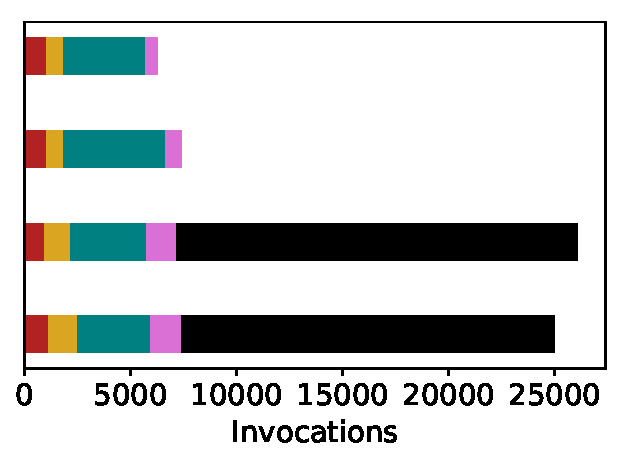
\includegraphics[width=0.17\textwidth]{../graphs/litmus_tests/faasbench_32_cold_hot.pdf}}
\caption{Impact of keep-alive on different function types.}
\label{fig:faasbench}
\end{figure}
\end{comment}

% Figure~\ref{fig:faasbench-stacked-32} shows the number of cold and dropped requests for the different functions, with a medium cache size of 32 GB.
% This setup is intended to evaluate our system in resource constrained environments.
% We see that dropped requests dominate, and FaasCache's more effective keep-alive serves 45\% of requests, while OpenWhisk only serving ~40\%.
% At the same time, warm starts improve 17\% using FaasCache.


Next, we use the skewed frequency workload and use functions from Table~\ref{tab:fc:workloads} to evaluate the impact on real applications. 
%The impact on the different function performances can be seen in Figure~\ref{fig:faasbench}.
To generate the workload, the CNN, DD, and Web-serving functions have an inter-arrival time of 1500 ms, and the Floating-point function has a lower IAT of 400 ms. 
%
Figure~\ref{fig:faasbench} shows the breakdown of different function invocations for this workload on a 48 GB server.
Interestingly, OpenWhisk drops a significant number (50\%) of requests due to the its high cold start overheads.
FaasCache increases the warm requests by more than $2\times$. 
Interestingly, the \emph{distribution} of warm starts is also different. 
FaasCache's Greedy-Dual policy prioritizes functions with higher initialization times, but penalizes those with large memory footprints. 
Because the floating-point function has a high initialization overhead (Table~\ref{tab:fc:workloads}), it sees a $3\times$ increase in hit-ratio compared to OpenWhisk.
\emph{In practical terms, the improvement in keep-alive results in a $6\times$ reduction in the application latency.
}
%The ML inference function has an 8\% lower warm hit rate than the other functions, as it gets de-prioritized because of it's high memory needs.


%When the cache size is increased to 48 GB (Figure~\ref{fig:faasbench-stacked-48}), FaasCache doesn't drop a single request, while OpenWhisk still can't serve 50\% of them.
%For the same workload, Figure~\ref{fig:faasbench-stacked-32} shows the distribution of cold and warm starts for a larger cache size of 32 GB.
%The number of warm starts increases by nearly 20\% compared to OpenWhisk.
% FaasCache's Greedy-Dual policy prioritizes functions with higher initialization times, the CNN function sees a 53\% higher warm starts, wheres Z function only sees X\% increase compared to OpenWhisk. 
% The floating point function has a very high initialization overhead (1.7 of the total 2 seconds), and thus sees its warm-start rate increase the most, by 40\%. 

\begin{comment}
At a smaller cache size of 32 GB shown in Figure~\ref{fig:faasbench-stacked-32}, the number of dropped requests dominate.
This setup is intended to evaluate our system in resource constrained environments.
FaasCache's more effective keep-alive serves 45\% of requests, while OpenWhisk drops nearly 60\%.
Warm-starts increase by 17\% with FaasCache. 
\end{comment}

\noindent \emph{\textbf{Result:} FaasCache can increase the number of warm-starts by $2\times$ to $3\times$ depending on the function initialization overheads and workload skew. This results in lower system load, which increases the number of requests FaasCache can serve by $2\times$.}

%\prat{CPU Graph not required, but just the average numbers will do.}

%%%%%%%%%%%%%%%%%%%%%%%%%%%%%%%%%%%%%%%%%%%%%%%%%%%%%%%%%%%%
\subsection{Effectiveness of Provisioning Policies}
All our previous results have been with a statically allocated server, and 
we now illustrate the effectiveness of our dynamic vertical scaling policy described in Section~\ref{subsec:dynamic}.
The goal is to dynamically adjust the cache size based on the workload. 
Our  policy seeks to keep the miss speed (cold starts per second) close to a pre-specified target. 
This is shown in Figure~\ref{fig:dynamic}---the target is 0.0015 misses per second. 
In this experiment, the cache resizing is done only when the miss speed error exceeds 30\%, and we can see that the cache size increases with the miss speed, and decreases with it. 
Without the dynamic scaling, a conservative provisioning policy would result in a constant, 10,000 MB size. 
In contrast, the average cache size with our proportional controller is less than 7,000 MB.
This 30\% reduction means that FaaS providers can reduce their provisioned resources without compromising on performance.
The freed-up resources can be used to accommodate additional cloud workloads (such as co-located VMs and containers). 
Our dynamic scaling is extremely conservative: increasing its agressiveness by reducing the error tolerance below 30\% will reduce  average server size,
%but cause a larger number of small memory-size  changes, which we wish to avoid.
but we seek to avoid the resultant small changes to memory-size to minimize fragmentation. 
%avoid why?? 

\begin{figure}[t]
  \centering 
  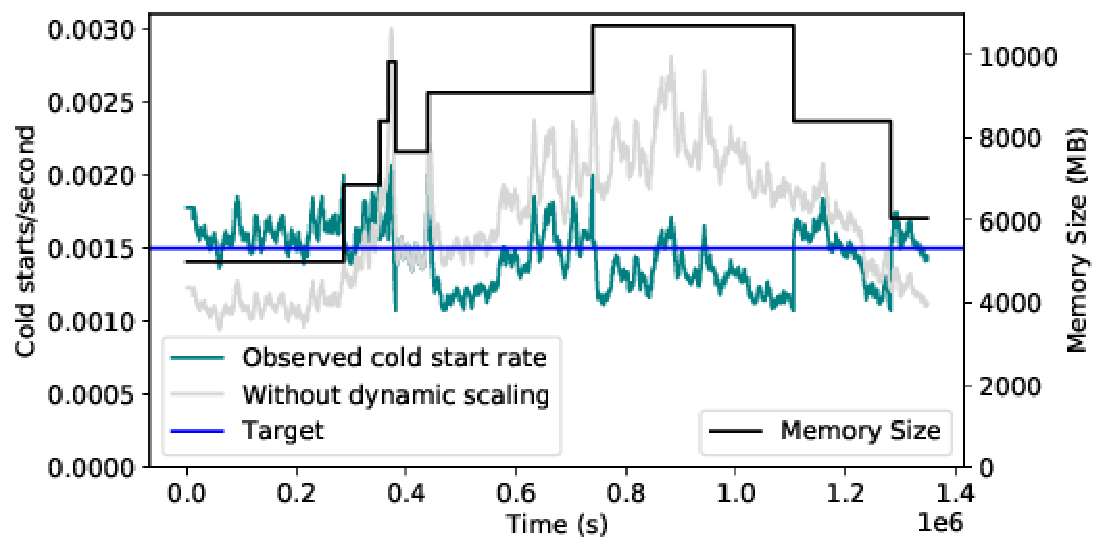
\includegraphics[width=0.6\textwidth]{faascache/faas-keepalive-20/graphs/dyn-scale-392-b.pdf}
  \caption{With dynamic cache size adjustment, the cold starts per second are kept close to the target (horizontal line), which reduces the average server size by 30\%. }
  \label{fig:dynamic}
\end{figure}

%%% Local Variables:
%%% mode: latex
%%% TeX-master: "paper"
%%% End:


\section{Related Work}
\section{Related Work}
\label{sec:related}

\noindent \textbf{Locality} is an important design and optimization principle in FaaS---and is a fundamental result of code and data initialization required for each function.
Keep-alive policies for warm-starts apply temporal locality~\cite{roy2022icebreaker, ebrahimi2024cold, vahidinia2022mitigating, shahrad2020serverless} and caching~\cite{faascache-asplos21, sundarrajan2017footprint} principles for the CPU memory pool; load balancing also benefits from stickiness~\cite{package-cristina-19, faaslb-hpdc22, abdi2023palette}.
Our work extends these principles to GPU functions via locality enhanced fair queuing and proactive memory management. 

% Bursty functions can cause load imbalance and queuing on systems, and intelligent queuing can avoid additional latency~\cite{yan2020hermes}.

\noindent \textbf{GPUs in serverless computing} is already a rich and fast-growing area of research. 
A big portion of prior work~\cite{naranjo2020accelerated, fingler2022dgsf, kim_gpu_2018} focuses on disaggregated accelerators, with GPUs accessed over the network using techniques such as rCUDA~\cite{duato2010rcuda}.
In contrast, we look at local GPUs without remote execution. 
Using FaaS-inspired abstractions to provide GPU acceleration as a service is also common: applications are broken down into kernels which can be run ``anywhere''.
Kernel-as-a-Service~\cite{pemberton2022kernel} and Molecule~\cite{du2022serverless} are two examples of this approach, where the main challenges are designing and providing efficient and usable API-remoting mechanisms. 
\cite{juan_reducing_2023} also uses remote memory pooling to address the exacerbated cold-start problems for GPUs, and also proposes parallel data-dependency and compute context prefetching through code-level optimizations. 
Paella~\cite{ng2023paella} similarly breaks apart model inference tasks into CUDA kernel launches to minimize scheduling ``bubbles''.
These and other recent~\cite{sage_zhao_towards_2024} specialized code-modifying techniques are orthogonal to our work, since we require general black-box functions.

% MIG Over-allocation causes fragmentation, and the opposite approach will reduce performance or prevent function execution due to insufficient resources.
% Assigned partitions can lead to underutilization due to fragmentation from poor placement and function idle periods. Idle functions cause immediate underutilization, which could be alleviated via temporal sharing complicating fixed hardware partition management even further.

The popularity of \textbf{ML inference} has resulted in a large number of specialized solutions to efficient GPU scheduling, which have similar challenges, but a different optimization spaces: inference resource requirements are much more deterministic~\cite{gujarati2020serving} and thus amenable to data-driven optimization~\cite{ali2022optimizing}, and the lack of isolation among requests provides many locality-enhancing and batching opportunities~\cite{yang2022infless, satzke2020efficient}. 
For instance, both FaST-GShare~\cite{gu2023fast} and TGS~\cite{tgs_wu2023transparent} leverage profiles of ML workloads to monitor GPU utilization and use 2d bin-packing (with time and memory dimensions) to schedule inference workloads.

%Both of these automatically move memory off of the device when kernels are done, and don't have to worry about applications holding onto device memory when idle.

%  profiles ML workloads to monitor how much of the GPU it utilizes, then uses this information to schedule inference tasks on GPUs to maximize utilization.
% ML inference tasks have fixed sized memory and kernel usages (known tensor sizes, etc.) and this is an effective approach.
% Other applications can have arbitrary and changing requirements, especially when one considers that function arguments are the main determiner of resource usage, so this idea breaks down when shifting to black-box applications.

Finally, \textbf{scheduling} is crucial for FaaS performance, with key tradeoffs in late vs. early binding~\cite{kaffes2021practical, kaffes_hermod_2022}.
Efficiency and fairness tradeoffs in GPU scheduling have been recently resolved~\cite{mo_optimal_2024}, but only in the offline context with a limited number of batch jobs with known utilities. 

%%% Local Variables:
%%% mode: latex
%%% TeX-master: "paper"
%%% End:


\bibliographystyle{plain}
\bibliography{faas}

% Moved to appendix-submit.tex
%\section{Appendix}
%\paragraph{OpenWhisk Evaluation Function Details.}


% The impact on the different function performances can be seen in Figure~\ref{fig:faasbench}.
% For this figure, to generate the workload, the first three functions have an inter-arrival time of 1500 ms, and the fourth (floating-point) has a lower IAT of 400 ms. 


We use the following functions from FunctionBench FaaS benchmark to run on OpenWhisk. 

\begin{enumerate}
  \item ML Inference: Image inference using the SqueezeNet CNN architecture, implemented in Tensorflow.
  \item Video Encoding: Download 11 MB mp4 file and convert it to a grayscale avi equivalent, using Python's cv2. 
  \item Matrix Multiplication: Using Numpy and \texttt{linalg.solve} of a randomly generated 20x20 matrix.
  \item Disk-bench: Read and write 1000 times from disk in 128k blocks using the \textbf{dd} command
  \item Web-serving: Generating and returning HTML for a small web page using Python's Chameleon. 
  \item Floating Point: A series of floating point trigonomotric computations using the standard Python math library.
\end{enumerate}



\paragraph{Azure Functions Dataset.}

We use the Azure function dataset to validate our keep-alive policies.
The full dataset consists of 14 days of function invocations, and billions of individual invocations. 
We use the first day's data, and do not consider functions with less than two invocations. 

Because memory is tracked at the \textit{application} level, and applications are made up of multiple functions, we evenly split the memory allocation between all functions in an application.


The dataset provides invocations in minute-wide buckets.
So when forming the traces, if there is only one invocation it is injected at the beginning of the minute.
For multiple invocations, they are equally spaced throughout the minute.

%Dataset location: https://github.com/Azure/AzurePublicDataset/blob/master/AzureFunctionsDataset2019.md

We use multiple different samples of this trace to validate our approach with different kinds of traces, and to make the analysis more tractable. We note that the full function trace is suitable for a large cluster of servers, whereas our focus is on a \emph{single} server.
The details of our trace samples are provided in Table~\ref{tab:trace-deets}. 
Figure~\ref{fig:whole-trace} shows the invocations/second of the full function trace (without sampling), and Figures~\ref{fig:392-trace}, \ref{fig:1000-trace}, and \ref{fig:200-trace} show the timeseries of our three workload traces. 
We can see that the representative trace (Figure~\ref{fig:392-trace}) captures the diurnal effects seen in the full trace (Figure~\ref{fig:whole-trace}).



\begin{table}
  \begin{tabular}{lrrr}
    \hline 
    Trace & Num Invocations & Reqs per sec & Avg. IAT \\
    \hline
    Representative & 1,348,162 & 190 /s & 5.4 ms \\
    Rare & 202,121 & 30 /s & 36 ms \\
    Random & 4,291,250 & 600 /s & 1.8 ms \\
    \hline
  \end{tabular}
  \caption{Size and IAT details for the three traces used in our evaluation.}
  \label{tab:trace-deets}
\end{table}


\begin{comment}

\begin{figure}[t]
  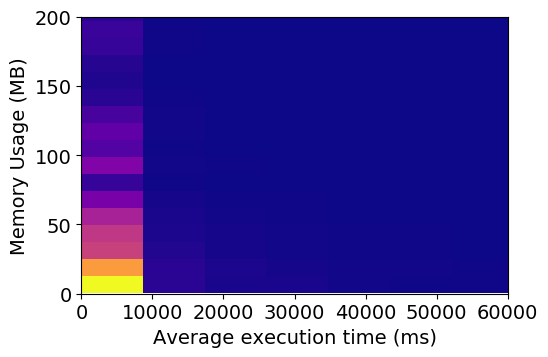
\includegraphics[width=0.3\textwidth]{../graphs/azure_analysis/mem-dur-corr.png}}
  \caption{Lack of correlation between a function's memory and average runtime duration}
  \label{fig:azure-mem-dur-corr}
\end{figure}

\begin{figure}[t]
  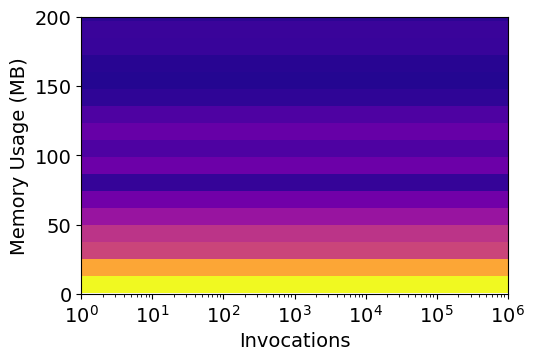
\includegraphics[width=0.3\textwidth]{../graphs/azure_analysis/mem-conv-corr.png}
  \caption{Lack of correlation between a function's memory and number of  times it is invoked}
  \label{fig:mem-invok-corr}
\end{figure}

\begin{figure}
    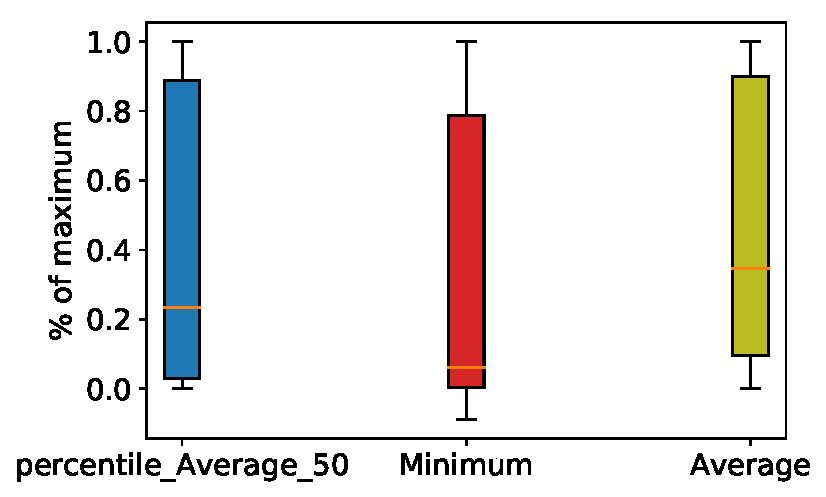
\includegraphics[width=0.3\textwidth]{../graphs/azure_analysis/cold_vs_warm.pdf}
    \caption{Relation between a functions maximum runtime and it's minimum, average, and 50th percentile average.}
    \label{fig:warm-cold-box}
\end{figure}

\end{comment}

\begin{figure}
 \centering 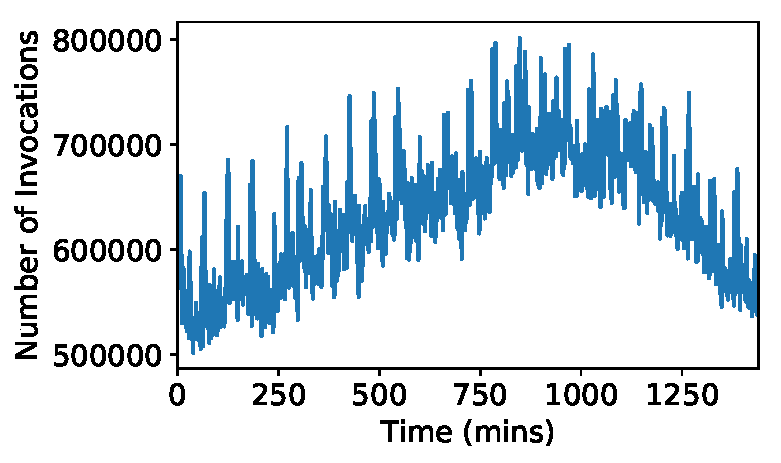
\includegraphics[width=0.3\textwidth]{../graphs/azure_analysis/whole_trace.pdf}
  \caption{Full Azure trace (Day 1) invocation timeseries.}
  \label{fig:whole-trace}
\end{figure}


\begin{figure}
 \centering   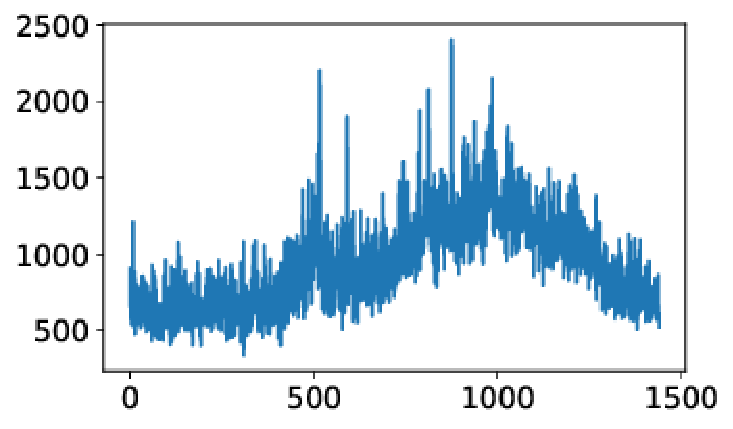
\includegraphics[width=0.3\textwidth]{../graphs/rep-funcs-392/392-b-trace.pdf}
  \caption{Representative trace invocation timeseries.}
  \label{fig:392-trace}
\end{figure}

\begin{figure}
  \centering  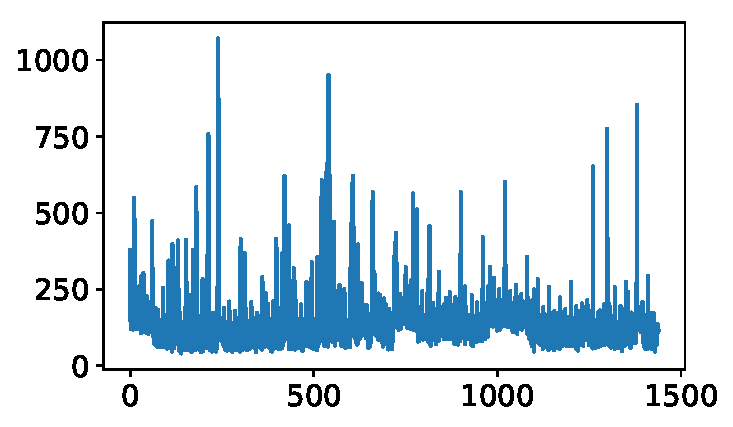
\includegraphics[width=0.3\textwidth]{../graphs/rare-funcs-1000/1000-b.pdf}
  \caption{Rare function trace invocation timeseries.}
  \label{fig:1000-trace}
\end{figure}


\begin{figure}
  \centering  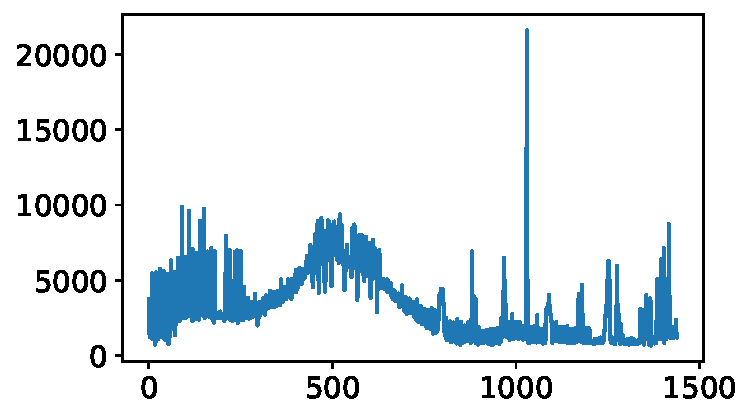
\includegraphics[width=0.3\textwidth]{../graphs/random-funcs-200/200-c.pdf}
  \caption{Randomly sampled trace invocation timeseries.}
  \label{fig:200-trace}
\end{figure}

%\end{comment}

%%% Local Variables:
%%% mode: latex
%%% TeX-master: "appendix-submit"
%%% End:


% LaTeX template for Artifact Evaluation V20201122
%
% Prepared by 
% * Grigori Fursin (cTuning foundation, France) 2014-2020
% * Bruce Childers (University of Pittsburgh, USA) 2014
%
% See examples of this Artifact Appendix in
%  * SC'17 paper: https://dl.acm.org/citation.cfm?id=3126948
%  * CGO'17 paper: https://www.cl.cam.ac.uk/~sa614/papers/Software-Prefetching-CGO2017.pdf
%  * ACM ReQuEST-ASPLOS'18 paper: https://dl.acm.org/citation.cfm?doid=3229762.3229763
%
% (C)opyright 2014-2020
%
% CC BY 4.0 license
%

%\pagebreak[4]
\clearpage
\section{Artifact Appendix}
% \appendix

%%%%%%%%%%%%%%%%%%%%%%%%%%%%%%%%%%%%%%%%%%%%%%%%%%%%%%%%%%%%%%%%%%%%%

\subsection{Artifact check-list (meta-information)}

{\small
\begin{itemize}
  \item {\bf Program: FaasCache }
  \item {\bf Data set: see~\ref{data-sets} }
  \item {\bf Run-time environment:  Ubuntu 16.04.5 }
  \item {\bf Hardware: 250 GB RAM, 48 cores }
  \item {\bf Experiments: Simulation \& OpenWhisk implementation }
  \item {\bf How much disk space required (approximately)?: 10 GB }
  \item {\bf How much time is needed to prepare workflow (approximately)?: 2 hours }
  \item {\bf How much time is needed to complete experiments (approximately)?: 6 hours }
  \item {\bf Publicly available?: Yes }
  \item {\bf Archived (provide DOI)?: 10.5281/zenodo.4321766 }
\end{itemize}

%%%%%%%%%%%%%%%%%%%%%%%%%%%%%%%%%%%%%%%%%%%%%%%%%%%%%%%%%%%%%%%%%%%%%
\subsection{Description}

We have two main software artifacts.

The first is a discrete-event simulator for FaaS workloads written in Python.
This simulator implements various keep-alive policies, all of which are described in the full paper.
Its inputs are workload trace files that are publicly available at the Azure trace site, and serialized into a custom format by scripts in {\em code/split/gen}.
The simulator takes server memory size, keep-alive policy, input trace file as arguments, and outputs various statistics on warm and cold starts, memory usage, and other accounting information. 
These outputs are run through the data-graphing scripts in {\em code/split/plotting}, to produce figures such as Figure 5 in the paper.

The second artifact is a custom OpenWhisk (i.e., FaasCache).
It is a drop-in replacement of OpenWhisk with the same installation procedures.
It optimizes OpenWhisk scheduling with GD keep-alive policy.
FaasCache or vanilla OpenWhisk can both be used to generate the information from Table 1 in the paper.

Our artifact also includes some FaasCache performance tests in {\em faas-keepalive/code/wsk-actions/load-test/traces}.
These can be run with scripts in {\em faas-keepalive/code/wsk-actions/load-test} that invoke LookBusy work-simulating FaaS functions at regular intervals to load test the FaasCache design.

Full details on how to run these two artifacts are in Section~\ref{experiments} below.
For brevity, portions talking about the simulator or OW load generation will be referencing folder {\em faas-keepalive}.
Those sections on running the customized OpenWhisk server are based in folder {\em openwhisk-caching}.

\subsubsection{How to access}

10.5281/zenodo.4321766

The code for both experiemts is in the zenodo zip, but also available on GitHub:

Simulator code is here:
https://github.com/aFuerst/faascache-sim

FaasCache OpenWhisk implementation:

https://github.com/aFuerst/openwhisk-caching/commit/38ff898d45da57726da38c00f735cb449e7f8595


\subsubsection{Hardware dependencies}

To reproduce the FaasCache load test results, you will nead 64 GB RAM, and 48 cpu cores for OW to use.
The simulator needs ~1 GB RAM/cpu, and will be made faster with higher number of parallel processes.


\subsubsection{Software dependencies}

\begin{enumerate}
  \item Python 3.7+
  \item Docker
  \item Java
\end{enumerate}


\subsubsection{Data sets} \label{data-sets}

https://github.com/Azure/AzurePublicDataset/

blob/master/AzureFunctionsDataset2019.md

The representative trace used in the paper is in the zip, called {\em 392-b.pckl}.
Pre-computed simulator results are also in the zip, in the folder {\em 392-pckls}. 
These are high-resolution results, memory-wise, as the simulation is compute-intensive (i.e. slow).

%%%%%%%%%%%%%%%%%%%%%%%%%%%%%%%%%%%%%%%%%%%%%%%%%%%%%%%%%%%%%%%%%%%%%
\subsection{Installation}

\subsubsection{Simulator Setup}

The original trace dataset can be found here:

https://github.com/Azure/AzurePublicDataset/

blob/master/AzureFunctionsDataset2019.md

The simulator code is available here, as well as in the zip:
https://github.com/aFuerst/faascache-sim

The script {\em ./code/split/trace\_split\_funcs.py} will combine the first day's info into one file.
Edit {\em datapath} and {\em store} in the script to adjust input and output locations.


{\em ./code/split/gen\_representative\_trace.py} will create traces that are generally representative of the larger trace sample.
Edit {\em datapath} and {\em store} in the script to adjust input for trace CSVs and split pickles (made by {\em trace\_split\_funcs.py} above) respectively.
{\em save\_dir} points to the folder where the resulting combined trace(s) will be saved.
Change lines 131-133 if you want specific trace sizes.

{\em ./code/split/gen\_rare.py} will create traces using the rarest half and quarter of functions.
You can edit line 99 to adjust which quartiles it picks functions from.
	

\subsubsection{FaasCache OpenWhisk Setup}

FaasCache OpenWhisk implementation:

https://github.com/aFuerst/openwhisk-caching/commit/38ff898d45da57726da38c00f735cb449e7f8595

Install the OpenWhisk CLI:

https://github.com/apache/openwhisk\#quick-start

OpenWhisk testing code: https://github.com/aFuerst/faascache-sim/tree/master/code/wsk-actions
(subset of FaasCache sim repo)

{\em core/containerpool/ContainerPool.scala} contains all the edits made to the OW source.


Have docker \& java installed
{\em ./code/wsk-actions/py/build.sh} will create zip packages for all the actions that OW can use.

To run the load tests on OpenWhisk you will also have to build the LookBusy Docker container in {\em ./code/wsk-actions/load-test/lookbusy}.
Make sure the new Docker container is added as a runtime to the OW {\em ansible/files/runtimes.json}.
The default AI container OW uses still may be missing packages, if this is the case you will also have to build the Dockerfile at {\em wsk-actions/py/cust\_ai} and add it as a custom runtime.

Edit the {\em ./sample-app.conf} in the root and put it in {\em ./bin/}.
Rename it to {\em application.conf}.
OW requires this configuration file to run and allow function creation.
You can adjust {\em container-pool.user-memory} depending on local resources.

{\em ./openwhisk-caching/blob/master/run.sh} will build and run the custom OpenWhisk.

Make sure the {\em .conf} {\em whisk.user} info matches between the scripts that talk to OW.

{\em code/wsk-actions/load-test/wsk\_interact.py} contains helper functions that interact with the OW CLI to set up functions and authentication.
If you use a different username or auth key then you will need to edit this file.

%%%%%%%%%%%%%%%%%%%%%%%%%%%%%%%%%%%%%%%%%%%%%%%%%%%%%%%%%%%%%%%%%%%%%
\subsection{Experiment workflow} \label{experiments}

\subsubsection{Run Simulator}

The {\em ./code/run\_sim.sh} file will run a trace in the simulator and graph the results.

\begin{enumerate}
  \item trace\_dir => folder where trace file needs to be
  \item trace\_output\_dir => folder where sim results will end up
  \item log\_dir => file where sim log data will end up
\end{enumerate}

The location pf the trace output and log output {\bf must} be different.

Edit the number of functions in {\em ./code/run\_sim.sh} to match the number of functions in the trace you want to run (this number will be in the file name).
Make sure the trace file letter (-b-, etc.) matches line 65 of {\em ./code/split/many\_run.py}, this is set by the trace generation script.

\subsubsection{Run FaasCache OpenWhisk}

You can follow the items in run.sh to run individual actions or run {\em ./code/wsk-actions/load-test/testing/find\_avgs.py} to get average run times for all the different actions.

{\em ./code/wsk-actions/load-test/gen\_litmus.py} will generate the litmus test pckls for the full OW tests.
Then run {\em code/wsk-actions/load-test/sub\_litmi.py} to invoke the litmus test.

Cold vs warm hit metrics are output to OW log (stdout from sh/jar). 
Make sure to pipe the output to a file.
You can grep on {\em cold hits:} to look at current results.

If you run the any of the litmus test, stop the test after 2 hours have past.
OW may or may not complete all invoked actions, stopping it significantly late is ok, just wastes time.
Then grep for the first hit event, record the time, then grep for the event closest to 2 hours later.
This will match how the paper results were gathered.

%%%%%%%%%%%%%%%%%%%%%%%%%%%%%%%%%%%%%%%%%%%%%%%%%%%%%%%%%%%%%%%%%%%%%
\subsection{Evaluation and expected results}

Results should be similar to those in the paper. 

The simulator results will not be exact if a new trace sampling is used, and if a coarser grained memory step is used.
The paper used 500 MB steps, but this dramatically increases needed simulation time.

Timings and numbers for the FaasCache OpenWhisk implementation will vary marginally due to the stochastic nature of web request handling and the inner workings of OW.


%%%%%%%%%%%%%%%%%%%%%%%%%%%%%%%%%%%%%%%%%%%%%%%%%%%%%%%%%%%%%%%%%%%%%
\subsection{Methodology}

Submission, reviewing and badging methodology:

\begin{itemize}
  \item \url{https://www.acm.org/publications/policies/artifact-review-badging}
  \item \url{http://cTuning.org/ae/submission-20201122.html}
  \item \url{http://cTuning.org/ae/reviewing-20201122.html}
\end{itemize}

\end{document}



%Hotcloud template... 


%%% Local Variables:
%%% mode: latex
%%% TeX-master: t
%%% End:
